\Subsection{Голоморфные функции}

Если доказательство не указано, то оно повторяет то, что было в $\mathbb{R}$ (смотреть 1 семестр).

\begin{definition}
    $\Omega$ -- обсласть в $\mathbb{C}, \ f: \Omega \rightarrow \mathbb{C}, \ z_0 \in \Omega$.

    $f$ -- голоморфна в точке $z_0$, если существует $\lim_{z \rightarrow z_0} { \frac{f(z) - f(z_0)}{z - z_0} } =: f'(z_0)$.
\end{definition}
\begin{definition}
    $f$ комплексно дифф. в точке $z_0$, если $\exists k \in \mathbb{C}$:

    $f(z) = f(z_0) + k (z - z_0) + o(z - z_0)$ при $z \rightarrow z_0$.
\end{definition}

\begin{statement}
    $f$ -- голоморфна в точке $z_0 \Leftrightarrow f$ комплексно дифф. в точке $z_0$ и $k = f'(z_0)$.
\end{statement}

\begin{consequence}
    $f$ и $g$ голоморфны в точке $z_0$. Тогда

    \begin{enumerate}
        \item {
            $f \pm g$ голом. в точке $z_0$
        }
        \item {
            $f \cdot g$ голом. в точке $z_0$
        }
        \item {
            Если $g(z_0 \not = 0)$, то $\frac{f}{g}$ голом. в точке $z_0$.
        }
        \item {
            Если $h$ голом. в точке $f(z_0)$, то $h \circ f$ голом. в точке $z_0$.
        }
    \end{enumerate}
\end{consequence}

\begin{remark}
    $f: \Omega \rightarrow \mathbb{C}$

    $z = x + iy, \ f(z) = f(x + iy) = g(x + i y) + i h(x + iy): \ g, h : \Omega \rightarrow \mathbb{R}$.

    $\frac{\partial f}{\partial x} (z_0) = \lim_{h \rightarrow 0, \ h \in \mathbb{R}} {\frac{f(z_0 + h) - f(z_0)}{h}} = f'(z_0)$.


    $\frac{\partial f}{\partial y} (z_0) = \lim_{h \rightarrow 0, \ h \in \mathbb{R}} {\frac{f(z_0 + i h) - f(z_0)}{h}} = \frac{f'(z_0)}{i} = i \cdot f'(z_0)$.
\end{remark}

\begin{remark}
    $\binom{g(x + iy)}{h(x + iy)} = \binom{g(x_0 + i y_0)}{h(x_0 + iy_0)} + \binom{a \ b}{c \ d} \binom{x - x_0}{y - y_0} + o(|| (x - x_0, y - y_0) ||)$.

    $k = \alpha + i \beta$

    $k \cdot (z - z_0) = (\alpha + i \beta) ( (x - x_0) + i (y - y_0)) = \alpha(x - x_0) - \beta(y - y_0) + i (\beta (x - x_0) + \alpha (y - y_0))$

    Вещественная линейность + $\binom{\alpha \ -\beta}{\beta \ \alpha} \Leftrightarrow$ комплескная линейность.
\end{remark}


% TODO: где-то есть места, где я пишу `\pi` и при этом забыто `\cdot i`, то есть надо `\pi \cdot i`. Это критическая ошибка, ее надо исправить !!!

\begin{remark}
    Комплескная дифференцируемость $\Leftrightarrow$ вещественная дифференцируемость + матрица Якоби $\binom{\alpha \ \beta}{-\beta \ \alpha}$


    Комплескная дифференцируемость $\Leftrightarrow$ вещественная дифференцируемость + условия Коши-Римана $
    \begin{cases}
        \frac{\partial Re(f)}{\partial x} = \frac{\partial Im (f)}{\partial y} \\
        \frac{\partial Re(f)}{\partial y} = -\frac{\partial Im (f)}{\partial x} \\
    \end{cases}
    $
\end{remark}
\begin{remark}
    $f(z) = f(z_0) + \underbrace{k}_{\in \mathbb{C}} (z - z_0) + o(z - z_0)$

    $k (z - z_0) = k w = |k| \cdot e^{i \phi} \cdot w, \ \phi = arg(k)$
\end{remark}


\begin{remark}
    Обозначения.

    $\frac{\partial}{\partial z} = \frac{1}{2} \cdot \left( \frac{\partial}{\partial x} - i \frac{\partial}{\partial y} \right)$

    $\frac{\partial}{\partial \overline{z}} = \frac{1}{2} \cdot \left( \frac{\partial}{\partial x} + i \frac{\partial}{\partial y} \right)$

    $dz = dx + i dy$

    $d \overline{z} = dx - i dy$

    $df = \frac{\partial f}{\partial x} \cdot dx + \frac{\partial f}{\partial y} dy = \frac{\partial f}{\partial z} dz + \frac{\partial f}{\partial \overline{z}} d \overline{z}$
\end{remark}

\begin{theorem}
    \textbf{Условия Коши-Римана}.

    $f: \Omega \rightarrow \mathbb{C}, \ a \in \Omega$

    $f$ -- дифф. в точке $a$ как функция из $\mathbb{R}^2$ в $\mathbb{R}^2$. Следующие условия равносильны:

    \begin{enumerate}
        \item {
            $f$ -- голоморфна в точке $a$.
        }
        \item {
            $d_a f$ -- комплексно линеен
        }
        \item {
            условия Коши-Римана
        }
        \item {
            $\frac{\partial f}{\partial \overline{z}} (a) = 0$
        }
    \end{enumerate}
\end{theorem}

\begin{proof}
    Мы выяснили все, кроме $(3) \Leftrightarrow (4)$:

    $\frac{\partial f}{\partial \overline{z}} = 0 \Leftrightarrow \frac{\partial f}{\partial x} + i \frac{\partial f}{\partial y} = 0 \Leftrightarrow \frac{\partial (Re(f) + i Im(f))}{\partial x} + i \cdot \frac{\partial (Re (f) + i Im (f))}{\partial y} = 0 \Leftrightarrow \begin{cases}
        \frac{\partial Re(f)}{\partial x} - \frac{\partial Im (f)}{\partial y} = 0 \\
        \frac{\partial Im(f)}{\partial x} + \frac{\partial Re(f)}{\partial y} = 0
    \end{cases}$ -- а это и есть условия Коши-Римана.
\end{proof}

\begin{remark}
    Обозначения.

    $f \in H(\Omega) \Leftrightarrow f : \Omega \rightarrow \mathbb{C}$ и голоморфна во всех точках из $\Omega$.
\end{remark}
\begin{consequence}
    $\Omega$ -- область, $f \in H(\Omega)$ и $Im(f) = const \implies f = const$
\end{consequence}
\begin{proof}
    $\frac{\partial Im (f)}{\partial y} = 0 \implies \frac{\partial Re(f)}{\partial x} = 0$

    $\frac{\partial Im (f)}{\partial x} = 0 \implies \frac{\partial Re(f)}{\partial y} = 0$

    $\implies Re(f) = const$
\end{proof}
\begin{theorem}
    \textbf{Коши} (ah, shit, here we go again...)

    $f \in H(\Omega) \implies $ форма $f(z) dz$ локально точная.
\end{theorem}
\begin{proof}
    Будет два разных док-ва.

    \begin{enumerate}
        \item {
            Для случая непрерывно-дифф. $\frac{\partial Re(f)}{\partial x}, \dots$ (имеются в виду все частные производные).

            Тогда замкнутость $\implies$ локальная точность.

            $f(z) dz = f(z) (dx + i dy) = (Re(f) + i \cdot Im(f)) \cdot (dx + i dy) = Re(f) dx - Im(f) dy + i (Im (f) dx + Re(f) dy)$.

            $P dx + Q dy$ -- замкн. $\Leftrightarrow \frac{\partial P}{\partial y} = \frac{\partial Q}{\partial x}$

            $Re(f) dx - Im(f) dy$ -- замкн. $\Leftrightarrow \frac{\partial Re(f)}{\partial y} = - \frac{\partial Im(f)}{\partial x}$

            $Im(f) dx + Re(f) dy$ -- замкн. $\Leftrightarrow \frac{\partial Im(f)}{\partial y} = \frac{\partial Re(f)}{\partial x}$
        }
        \item {
            Общий случай.

            Надо доказать, что интеграл по любому прямоугольнику со сторонами параллельными осям координат из шарика $U \subset \Omega$, содержащего произвольную точку, равен 0.

            От противного: пусть нашелся прямоугольник $P$, т.ч. $\alpha (P) := \int_P {f(z) dz } \not = 0$.

            \begin{center}
                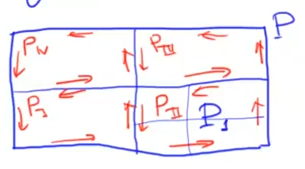
\includegraphics[width=7cm]{assets/04-functions-of-complex-variables/Cauchy-theorem-rectangle-partition.png}
            \end{center}


            Режем прямоугольник на 4 части, индексируем как $P^{1}, P^{2}, P^{3}, P^{4}$, строим обходы каждого (против часовой стрелки). Тогда $\alpha(P) = \alpha(P^{1}) + \alpha(P^{2}) + \alpha(P^{3}) + \alpha(P^{4})$, $|\alpha(P)| \leq |\alpha(P^{1})| + |\alpha(P^{2})| + |\alpha(P^{3})| + \alpha(P^{4})$.

            Хотя бы одно из слагаемых $\geq \frac{1}{4} |\alpha(P)|$, назовем такое $P_1$ (индекс уже снизу!). Разрежем его на 4 равные части. Пусть $P_2$ такой, что $|\alpha(P_2)| \geq \frac{1}{4} |\alpha (P_1)|$ и т.д.

            $|\alpha(P_n)| \geq \frac{1}{4^n} |\alpha (P)|$.

            % todo: picture
            \begin{center}
                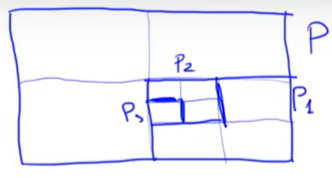
\includegraphics[width=7cm]{assets/04-functions-of-complex-variables/Cauchy-theorem-rectangle-partition-2.png}
            \end{center}

            Берем $a$ из $P_n$:

            $f(z) = f(a) + f'(a) (z - a) + o(z - a)$

            $\alpha (P_n) = \int_{P_n} { f(z) dz } = \underbrace{\int_{P_n} { f(a) dz }}_{= 0 \text{, по 1-ому док-ву}} + \underbrace{\int_{P_n} { f'(a) (z - a) dz }}_{= 0 \text{, по 1-ому док-ву}} + \int_{P_n} { o(z - a) dz }$


            \begin{center}
                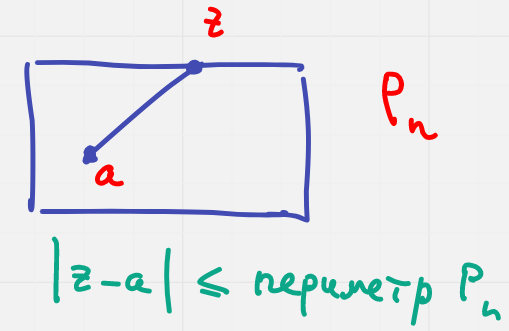
\includegraphics[width=7cm]{assets/04-functions-of-complex-variables/Cauchy-theorem-rectangle-partition-3.png}
            \end{center}


            $o(z - a) = (z - a) \cdot \beta (z - a)$, где $\beta(z - a) \underbrace{\rightarrow}_{z \rightarrow a} 0$

            $\left| \int_{P_n} {(z - a) \beta (z - a) dz} \right| \leq max_{z \in P_n} { |z - a| \cdot |\beta (z - a)| } \cdot \underbrace{l(P_n)}_{\text{периметр}} \leq max_{z \in P_n} { |\beta (z - a)| } \cdot \frac{l(P)}{2^n} \cdot \frac{l(P)}{2^n} \implies$

            $\implies \frac{|\alpha (P)|}{4^n} \leq |\alpha(P_n)| \leq \frac{l(P) \cdot l(P)}{4^n} \cdot max_{z \in P_n} |\beta (z - a)| \implies max_{z \in P_n} |\beta (z - a)| \geq \frac{|\alpha (P)|}{l(P) \cdot l(P)} > 0$ -- противоречие, т.к. $\beta(z) \rightarrow 0$ при $z \rightarrow a$.
        }
    \end{enumerate}
\end{proof}
\begin{consequence}
    \begin{enumerate}
        \item {
            Если $f \in H(\Omega)$, то у каждой точки $a \in \Omega$ есть окрестность, в которой существует ф-я $F$, т.ч. $F' = f$ в этой окрестности.

            \begin{proof}
                Пусть $F$ первообразная формы $f(z) dz$. Поймем, что $F' = f$.

                $\frac{\partial F}{\partial x} = f(z), \ \frac{\partial F}{\partial y} = i \cdot f(z) \implies \frac{\partial F}{\partial x} + i \frac{\partial F}{\partial y} = 0 \implies \frac{\partial F}{\partial \overline{z}} = 0$
            \end{proof}
        }
        \item {
            $f \in H(\Omega)$, $\gamma$ стягиваемый в $\Omega$ путь $\implies \int_{\gamma} { f(z) dz } = 0$
        }
    \end{enumerate}
\end{consequence}
\begin{theorem}
    $f \in C(\Omega), \ \Delta$ -- прямая параллельная оси координат.

    $f \in H(\Omega \setminus \Delta)$

    Тогда $f(z) dz$ локально точная.
\end{theorem}

\begin{proof}
    Надо проверять, что интеграл по довольно маленькому прямоугольнику (со стороронами паралл. осям) это 0.

    \begin{center}
        \includegraphics*[width=0.3\textwidth]{assets/04-functions-of-complex-variables/interesting-rectangles-locally-exact-form-without-line.png}
    \end{center}

    Очевидно, что если прямоугольник не пересекает $\Delta$, то там все очевидно. Хотим рассматривать только те, что задевают. Те, что пересекают $\Delta$, можно разбить на две части (верхнюю и нижнюю). По каждой из частей будет 0, тогда и в сумме тоже будет 0. То есть нас вообще интересуют только те прямоугольники, у которых $\Delta$ это одна из сторон. Рассмотрим их:

    \begin{center}
        \includegraphics*[width=0.5\textwidth]{assets/04-functions-of-complex-variables/smaller-rectangle-locally-exact-form-without-line.png}
    \end{center}

    $\int_{P_{\epsilon}} { f(z) d z } = 0 \rightarrow_{\epsilon \rightarrow 0} \int_{P} { f(z) dz }$

    $\left|\int_{P} {f(z) dz} - \int_{P_{\epsilon}} { f(z) dz } \right| \leq |\int_{1} + \int_{3}| + |\int_{2}| + |\int_{4}|$

    $\left| \int_{2} {f(z) dz} \right| \leq M \cdot (\text{длина } 2) = M \epsilon$

    $\left| \int_{1} + \int_{3} \right| = \left| \int_{a}^{b} { \left(f (x + i y_0) - f(x + i(y_0 + \epsilon)) \right) dx } \right| \leq \int_{a}^{b} { |\dots| dx } = (*)$

    $f$ непрер. на компакте $\implies$ равномерно непрер.

    $\forall \gamma > 0: \ \exists \epsilon > 0$ если $\rho (\text{аргумент}) < \epsilon \implies |f(\dots) - f(\dots)| < \gamma$, тогда

    $(*) \leq (b - a) \cdot \gamma$
\end{proof}

\begin{consequence}
    $f: \Omega \rightarrow \mathbb{C}$

    $f \in C(\Omega)$ и $f$ голоморфна в $\Omega$ за исключением мн-ва изолированных точек, тогда форма $f(z) dz$ все равно лок. точная.
\end{consequence}
\begin{proof}
    Рассмотрим окр-ть, в которой ровно одна плохая точка.

    % todo: picture
    Давайте проведем прямую через это точку, тогда работает теорема.
\end{proof}

\begin{definition}
    Индекс кривой отн-но точки $Ind(\gamma, z_0)$.

    $\gamma$ -- замкнутая кривая, не проходящая через точку $z_0$.

    $Ind(\gamma, 0) = \frac{\phi(b) - \phi(a)}{2\pi} \in \mathbb{Z}$ -- кол-во оборотов $\gamma$ вокруг 0.

    $\gamma: [a, b] \rightarrow \mathbb{C}$

    $\gamma(t) = r(t) e^{i \phi(t)}$, $\phi$ -- непрерывна (полярная замена).
\end{definition}

\begin{theorem}
    Пусть $\gamma$ -- замкнутая кривая, не проходящая через 0. Тогда

    $\int_{\gamma} { \frac{d z}{z} } = 2\pi i Ind(\gamma, 0)$.
\end{theorem}
\begin{proof}
    Берем параметризацию $r, \phi: [a, b] \rightarrow \mathbb{R}$

    $z(t) = r(t) e^{i \phi(t)}, \ dz = \left( r' e^{i\phi} + ri \phi' e^{i\phi} \right) dt$

    $\frac{dz}{z} = \frac{r'}{r} + i \phi'$

    $\int_{\gamma} { \frac{dz}{z} } = \int_{a}^{b} { \left( \frac{r'(t)}{r(t)} + i \phi'(t) \right) dt } = \left( ln (r(t)) + i \phi(t) \right)|_{t = a}^{t = b} = i (\phi(b) - \phi(a)) = 2 \pi i Ind(\gamma, 0)$
\end{proof}

\begin{consequence}
    Пусть $\gamma$ -- замкнутая кривая, не проходящая через точку $a$. Тогда

    $\int_{\gamma} { \frac{dz}{z - a} = 2 \pi i Ind (\gamma, a) }$.
\end{consequence}

\begin{theorem}
    (интегральная формула Коши).

    $f \in H(\Omega)$

    $\gamma$ -- стягиваемая в $\Omega$ кривая, не проходящая через $a \in \Omega$.

    Тогда $\int_{\gamma} { \frac{f(z) dz}{z - a} } = 2 \pi i f(a) Ind(\gamma, a)$
\end{theorem}
\begin{proof}
    $g(z) = \begin{cases}
        \frac{f(z) - f(a)}{z - a}, \ \text{при } z \not = a, \\
        f'(a), \ \text{иначе}
    \end{cases}$

    $g \in C(\Omega)$

    $g \in H(\Omega \setminus \{ a \})$

    $\implies g(z) dz$ -- локально точкая форма $\implies \int_{\gamma} {g(z) dz} = 0$, так как $\gamma$ -- стягиваемая

    $\implies 0 = \int_{\gamma} { \frac{f(z) dz}{z - a} } - \int_{\gamma} { \frac{f(a) dz}{z - a} } \implies \int_{\gamma} { \frac{f(z) dz}{z - a} } = f(a) \cdot \int_{\gamma} { \frac{dz}{z - a} } = f(a) \cdot 2 \pi i \cdot Ind(\gamma, a)$
\end{proof}
\begin{example}
    % todo: picture !!!
    Берем круг. $f$ -- голоморфна в окр-ти этого круга.

    $\int_{\text{окр.}} { \frac{f(z)}{z - a} dz } = \begin{cases}
        0, \ \text{ если $a$ вне круга} \\
        f(a) \cdot 2 \pi i, \ \text{ если $a$ внутри круга }
    \end{cases}$
\end{example}

\begin{remark}
    Обозначение.

    $\mathbb{D} = \{ |z| \leq 1 \}$ -- единичный круг.

    $\mathbb{T} = \{ |z| = 1 \}$ -- единичная окружность, обход против часовой стрелки.

    $r\mathbb{T} + a = \{ |z - a| = r \}$
\end{remark}

\begin{theorem}
    $f \in H(r \mathbb{D}) \implies f$ аналитична ($=$ функция раскладывается в ряд) в этом круге.
\end{theorem}

\begin{proof}
    % todo: picture
    В нашем круге радиуса $r$ берем еще два круга с тем же центром, но меньшими радиусами ($r > r_1 > r_2 > 0$). Берем $z: \ |z| < r_2$ -- точка внутри наименьшего круга. Хотим интегрировать по средней окружности.

    $f(z) = \frac{1}{2 \pi i} \int_{r_1 \mathbb{T}} { \frac{f(\zeta) d \zeta }{\zeta - z} }$

    $\frac{1}{\zeta - z} = \frac{1}{1 - \frac{z}{\zeta}} \cdot \frac{1}{\zeta} = \sum_{n=0}^{\infty} \frac{z^n}{\zeta^{n+1}} = (*)$ равномерно сх-ся, так как $\left| \frac{z}{\zeta} \right| \leq \frac{r_2}{r_1} < 1$

    $(*) = \frac{1}{2\pi i} \int_{r_1 \mathbb{T}} { \sum_{n=0}^{\infty} \frac{f(\zeta)}{\zeta^{n+1}} z^n d\zeta } = \frac{1}{2\pi i} \sum_{n=0}^{\infty} z^n \underbrace{\int_{r_1 \mathbb{T}} {\frac{f(\zeta)}{\zeta^{n+1}} d\zeta}}_{=: a_n \cdot 2\pi i} = \sum_{n=0}^{\infty} {a_n z^n}$
\end{proof}



\begin{consequence}
    \begin{enumerate}
        \item {
            Если $f \in H(r \mathbb{D})$ и $0 < r_1 < r$, то

            $\frac{n!}{2 \pi i} \cdot \int_{r_1 \mathbb{T}} { \frac{f(z)}{z^{n+1}} dz } = f^{(n)} (0)$
        }
        \item {
            $f \in H(r \mathbb{D} + a), \ 0 < r_1 < r \implies \frac{n!}{2 \pi i} \int_{r_1 \mathbb{T} + a} { \frac{f(z)}{(z - a)^{n + 1}} dz } = f^{(n)} (a)$

            $z = w + a$

            $g(w) = f(w + a)$

            $g^{(n)} (0) = \frac{n!}{2 \pi i} \cdot \int_{r_1 \mathbb{T}} { \frac{g(w)}{w^{n + 1}} dw }$
        }
        \item {
            $f: \Omega \rightarrow \mathbb{C}$

            Тогда $f$ -- голоморфна в $\Omega \Leftrightarrow f$ -- аналитична в $\Omega$.

            % todo: picture
        }
        \item {
            $f \in H(\Omega) \implies f$ -- бесконечно диффиренцируема.
        }
        \item {
            $f \in H(\Omega) \implies f' \in H(\Omega)$
        }
        \item {
            \begin{definition}
                $g: \mathbb{R}^n \rightarrow \mathbb{R}$ -- гармоническая, если $\frac{\partial^2 g}{\partial x_1^2} + \frac{\partial^2 g}{\partial x_2^2} + \dots + \frac{\partial g}{\partial x_n^2} = 0$.
            \end{definition}

            Продолжаем свойство:

            $f \in H(\Omega) \implies Re (f)$ и $Im(f)$ -- гармонические функции.

            \begin{proof}
                $\frac{\partial^2 Re(f)}{\partial x^2} = \frac{\partial}{\partial x} \left( \frac{\partial Re (f)}{\partial x} \right) = \frac{\partial}{\partial x} \left( \frac{\partial Im(f)}{\partial y} \right) = \frac{\partial}{\partial y} \left( \frac{\partial Im(f)}{\partial x} \right) = \frac{\partial}{\partial y} \left( - \frac{\partial Re(f)}{\partial y} \right) = - \frac{\partial^2 Re(f)}{\partial y^2}$

                про $Im(f)$ аналогично доказывается.
            \end{proof}
        }
    \end{enumerate}
\end{consequence}

\begin{remark}
    Если $g: \Omega \rightarrow \mathbb{R}$ гармоническая ф-я, то существует единств. (с точностью до прибавления $const \in \mathbb{R}$) гармоническая ф-я $h: \Omega \rightarrow \mathbb{R}$, т.ч. $g + i h \in H(\Omega)$
\end{remark}

\begin{theorem}
    \textbf{Мореры}.

    $f \in C(\Omega)$. Если $f(z) dz$ локально точная, то $f \in H(\Omega)$.
\end{theorem}
\begin{proof}
    Возьмем $a \in \Omega$. Существует окр-ть $a$, что для $f$ в ней есть первообразная $F$ (т.е. $F' = f$ в $U$).

    Тогда $F \in H(U) \implies F' = f \in H(U)$ -- это локальное свойство, поэтому на всей $\Omega$ тоже будет гомоморфность.
\end{proof}

\begin{consequence}
    $f \in C(\Omega), \ \Delta$ -- прямая, параллельная оси координат.

    $f \in H(\Omega \setminus \Delta)$. Тогда $f \in H(\Omega)$.
\end{consequence}
\begin{proof}
    $f \in C(\Omega)$ и $f \in H(\Omega \setminus \Delta) \implies f(z) dz$ локально точная в $\Omega \underbrace{\implies}_{\text{т. Мореры}} f \in H(\Omega)$.
\end{proof}

\begin{theorem}
    (интегральная формула Коши).

    $f \in H(\Omega)$

    $K \subset \Omega$ -- компакт, граница которого -- конечное число кусочно-гладких замкнутых кривых. Тогда

    \begin{enumerate}
        \item {
            $\int_{\partial K} { f(z) dz } = 0$
        }
        \item {
            Если $a \in Int (K)$, то $\int_{\partial K} { \frac{f(z)}{z - a} dz } = 2 \pi i f(a)$.
        }
    \end{enumerate}
\end{theorem}
\begin{proof}
    \begin{enumerate}
        \item {
            Пишем \textbf{формулу Грина}.

            $\int_{\partial K} { f(z) dz } = \int_{\partial K} { f(z) dx + i \cdot f(z) dy } \underbrace{=}_{\text{Грин}} \int_{K} { \left( i \cdot \frac{\partial f}{\partial x}  - \frac{\partial f}{\partial y} \right) dx dy } = $

            $ = i \cdot \int_{K} {\left( \frac{\partial f}{\partial x} + i \frac{\partial f}{\partial y} \right) dx dy} = 2 i \int_{K} { \frac{\partial f}{\partial \overline{z}} d \lambda_2 } = 0$.
        }
        \item {
            % todo: picture !!!
            Берем круг, содержащий $a$, не вылезающий за границу формы $B_r(a)$.

            $\tilde{K} = K \setminus B_r(a)$ -- компакт.

            $\frac{f(z)}{z - a} \in H(\Omega \setminus \{ a \}), \ \tilde{K} \subset \Omega \setminus \{ a \}$.

            $0 = \int_{\partial \tilde{K}} { \frac{f(z)}{z - a} dz } = \int_{\partial K} { \frac{f(z)}{z - a} dz } - \underbrace{\int_{r \mathbb{T} + a} { \frac{f(z)}{z - a} dz }}_{= 2\pi i f(a)}$.
        }
    \end{enumerate}
\end{proof}
\begin{exerc}
    $f \in H(r \mathbb{D})$ и $f \in C(Cl (r \mathbb{D}))$

    $a \in \mathbb{D}$.

    Доказать, что $\int_{r \mathbb{T}} { \frac{f(z)}{z - a} dz } = 2 \pi i f(a)$
\end{exerc}

\begin{theorem}
    $f \in C(\Omega)$. Следующие условия равносильны (равносильность всех утверждений, так или иначе, уже доказывалась ранее):

    \begin{enumerate}
        \item {
            $f \in H(\Omega)$
        }
        \item {
            $f(z) dz$ -- локально точная в $\Omega$
        }
        \item {
            В окр-ти каждой точки у $f$ есть первообразная
        }
        \item {
            $f$ аналитична в $\Omega$
        }
        \item {
            $\int{f(z) dz} = 0$ по любому достаточно малому прямоугольнику со сторонами параллельными осям
        }
        \item {
            $f(z) dz$ -- замкнутая и частн. производные по $x$ и $y$ непрерывны.
        }
    \end{enumerate}
\end{theorem}

\begin{theorem}
    \textbf{Неравенство Коши}.

    $f \in H(R \mathbb{D}), \ 0 < r < R$.

    $f(z) = \sum_{n=0}^{\infty} {a_n z^n}$. Тогда $|a_n| \leq \frac{M(r)}{r^n}$, где $M(r) := \max_{|z| = r} |f(z)|$.
\end{theorem}
\begin{theorem}
    $a_n = \frac{1}{2 \pi i} \int_{|z| = r} { \frac{f(z)}{z^{n + 1}} dz }$

    $|a_n| = \frac{1}{2 \pi} \left| \int_{|z| = r} { \frac{f(z)}{z^{n+1}} dz } \right| \leq \frac{1}{2 \pi} \cdot \max_{|t| = r} \left|\frac{f(z)}{z^{n+1}}\right| \cdot 2 \pi r = \frac{M(r)}{r^{n + 1}} \cdot r = \frac{M(r)}{r^n}$
\end{theorem}

\begin{theorem}
    \textbf{Луивилля}.

    Если $f \in H(\mathbb{C})$ и $f$ -- ограничена, то $f = const$.
\end{theorem}
\begin{proof}
    $f$ -- ограничена $\implies |f| \leq M$.

    $f \in H(\mathbb{C}) \implies f(z) = \sum_{n=0}^{\infty} { a_n z^{n} }$ и ряд сходится $\forall z \in \mathbb{C} \underbrace{\implies}_{\text{нер-во Коши}} |a_n| \leq \frac{M_r}{r^n} \leq \frac{M}{r^n} \underbrace{\rightarrow}_{r \rightarrow +\infty} 0 \implies a_n = 0: \ \forall n \geq 1$
\end{proof}

\begin{remark}
    $\sin$ и $\cos$ неограничены в $\mathbb{C}$.
\end{remark}

\begin{definition}
    Целая функция -- функция, голоморфная в $\mathbb{C}$.
\end{definition}

\begin{theorem}
    \textbf{Основная теорема алгебры}.

    $P$ -- многочлен степени $\geq 1$. Тогда у $P$ есть хотя бы один корень.
\end{theorem}
\begin{consequence}
    Если $deg P = n$, то $P(z) = c(z - z_1)(z - z_2) \dots (z - z_n)$ для некоторых $z_1, z_2, \dots z_n \in \mathbb{C}$.
\end{consequence}
\begin{proof}
    Если $z_1$ -- корень $P$, то $P(z) = (z - z_1) \cdot Q(z)$, где $deg Q = n - 1$.
\end{proof}
\begin{proof}
    Основной теоремы алгебры.

    От противного:

    пусть $P(z) \not = 0 \ \forall z \in \mathbb{C}$. Тогда $f(z) = \frac{1}{P(z)} \in H(\mathbb{C})$.

    Докажем, что $f$ -- ограниченная функция.

    $P(z) = z^n + a_{n-1} z^{n-1} + \dots + a_1 z + a_0$

    $R := 1 + |a_{n-1}| + |a_{n-2}| + \dots + |a_1| + |a_0|$. Пусть $|z| \geq R, \ |P(z)| \geq |z|^n - |a_{n-1}| |z|^{n-1} - \dots - |a_1| |z| - |a_0| \geq |z|^n - |z|^{n-1} (|a_{n-1}| + |a_{n-2}| + \dots + |a_0|) = \underbrace{|z|^{n-1}}_{\geq 1} \underbrace{(|z| - |a_0| - |a_1| - \dots - |a_{n-1}|)}_{\geq 1} \implies |P(z)| \geq 1$ при $|z| \geq R \implies |f(z)| \leq 1$ при $|z| \geq R$.

    Докажем, что при $|z| \leq R, \ |f(z)|$ -- ограничена.

    $f \in H(\mathbb{C}) \implies f$ непрер. в $\mathbb{C} \implies f$ непрер. в $\{ |z| \leq R \}$ -- компакт $\implies |f|$ огр. в $\{ |z| \leq R \}$.

    Тогда по т. Луивиля $f(z) = const \implies P(z) = \frac{1}{const}$, что противоречит условию, что $P(z)$ -- многочлен степени $\geq 1$.
\end{proof}


\Subsection{Теоремы единственности}
\begin{theorem}
    $f \in H(\Omega)$, $\Omega$ -- область, $z_0 \in \Omega$. След. условия равносильны:

    \begin{enumerate}
        \item {
            $f^{(n)} (z_0) = 0 \ \forall n = 0, 1, 2, \dots$
        }
        \item {
            $f = 0$ в некоторой окр-ти точки $z_0$.
        }
        \item {
            $f \equiv 0$ в $\Omega$
        }
    \end{enumerate}
\end{theorem}


\begin{lemma}
    $\Omega$ -- область в метрическом пространстве, $E \subset \Omega$, т.ч. $E \not = \emptyset, \ E$ -- открыто в $\Omega$, $E$ -- замкнуто в $\Omega$. Тогда $E = \Omega$.
\end{lemma}
\begin{proof} Леммы.

    Пусть $\Omega \setminus E \not = \emptyset$, берем $a \in E$ и $b \in \Omega \setminus E$. Возьмем путь $\gamma$, соединяющий эти точки.

    $\gamma: [\alpha, \beta] \rightarrow \Omega$, т.ч. $\gamma(\alpha) = a, \ \gamma(\beta) = b$. $\gamma$ -- непрер. $\implies \gamma^{-1} (E)$ -- открыто, $\gamma^{-1}(\Omega \setminus E)$ -- открыто $\implies \gamma^{-1}(E)$ -- открыт. и замкнут. подмн-во $[\alpha, \beta], \ \alpha \in \gamma^{-1}(E), \ \beta \not \in \gamma^{-1}(E)$.

    $s := \sup{\gamma^{-1} (E)}$ из замкн. $s \in \gamma^{-1} (E) \implies s < \beta$.

    % todo: picture

    Возьмем окр-ть $s$, т.ч. $(s - \delta, s + \delta) \subset \gamma^{-1}(E) \cap (\alpha, \beta) \implies $ в $\gamma^{-1}(E)$ есть точки $> s \implies s $ не $\sup$. Противоречие.
\end{proof}

\begin{proof}
    Теоремы.

    $(3) \implies (2) \implies (1)$ -- очевидно.

    $(1) \implies (2)$ -- почти очевидно:

    % todo: picture
    Берем $z_0 \in \Omega$ и $B_r(z_0) \subset \Omega$, тогда в круге $|z - z_0| < r: $ $f$ раскл. в свой ряд Тейлора $\implies$ в нем $f \equiv 0$.

    $(2) \implies (3)$:

    $E := \{ z \in \Omega: \ \text{в некоторой окр-ти точки } z, \ f = 0 \}$

    $z_0 \in E$ по условию $\implies E \not = \emptyset$.

    $E$ -- открыто. Если $w \in E$, то в круге $|z - w| < r, \ f = 0$.
    % todo: picture

    $\forall z$ из этого круга есть круг меньшего радиуса, содерж. $\{ |z - w| < r \}$, в нем $f = 0$.

    $E$ -- замкнуто. Пусть $z_*$ -- предельная точка $E$, то есть $z_n \in E$ и $\lim{z_n} = z_*$. $f^{(m)} (z_n) = 0 \ \forall m, \ \forall n$ (так как есть $(2) \implies (1)$). По непрерывности $f^{(m)} \ f^{(m)} (z_*) = \lim{f^{(m)} (z_n)} = 0 \underbrace{\implies}_{(1) \implies (2)} z_* \in E$.

    Тогда по лемме $E = \Omega$.
\end{proof}


\begin{consequence}
    $f, g \in H(\mathbb{C})$, т.ч. $f(z) = g(z)$ в окр-ти точки $z_0 \in \Omega \implies f \equiv g$.
\end{consequence}



\begin{theorem}
    \textbf{О среднем}.

    $f \in H(\Omega)$ и $a \in \Omega$, причем $\{ |z - a| \leq r \} \subset \Omega$, тогда $f(a) = \frac{1}{2\pi} \cdot \int_{0}^{2\pi} { f(a + r e^{i \phi}) d \phi }$ (т.е. среднее значение на окружности радиуса $r$ с центром в $a$ равно $f(a)$).
\end{theorem}
\begin{proof}
    $f(a) = \frac{1}{2 \pi i}\int_{|z - a| = r}{ \frac{f(z)}{z - a} dz } = \frac{1}{2 \pi i} \int_{0}^{2\pi} { \frac{f(a + r e^{i \phi})}{r e^{i \phi}} r e^{i \phi} i d \phi }$, где $z = a+re^{i\phi}, \ dz = r e^{i \phi} i d \phi$.
\end{proof}

\begin{consequence}
    $f \in H(\Omega), \ a \in \Omega, \ \{ |z - a| \leq r \} \subset \Omega$. Тогда $f(a) = \frac{1}{\pi r^2} \int_{|z-a|\leq r} { f(z) d \lambda_2 }$.
\end{consequence}
\begin{proof}
    $\int_{|z-a| \leq r} { f(z) d \lambda_2 } = \int_{0}^{r} { \int_{0}^{2\pi} {f(a + \rho e^{i\phi}) \rho d \phi } d \rho } = \int_{0}^{r} { 2 \pi f(a) \rho \ d \rho } =$

    $= 2 \pi f(a) \frac{r^2}{2} = \pi r^2 f(a)$.
\end{proof}

\begin{theorem}
    \textbf{Принцип максимума}.

    $f \in H(\mathbb{C}), \ a \in \Omega$. Если $|f(a)| \geq |f(z)| \ \forall z$ из окр-ти точки $a$, то $f \equiv const$.
\end{theorem}
\begin{proof}
    Пусть $|f(a)| =: M$. Домножим $f$ на $e^{i \alpha}$ так, что $f(a) = M > 0$.

    $|f(a)| = M = \frac{1}{2\pi} \left|\int_{0}^{2\pi} { f(a + r e^{i \phi}) d \phi }\right| \leq \frac{1}{2 \pi} \int_{0}^{2\pi} { |f(a + r e^{i \phi})| d \phi} \leq \frac{1}{2\pi} \int_{0}^{2\pi} { M \ d \phi } = M$.

    Все нер-ва обращаются в равенства $\implies |f(a + r e^{i \phi})| = M \ \forall \phi \ \forall$ маленьких $r$.

    $Re (f(a)) = M = \frac{1}{2\pi} \int_{0}^{2\pi} { Re(f(a + r e^{i \phi})) d \phi } \leq \frac{1}{2 \pi} \int_{0}^{2\pi} { |f(a + r e^{i \phi})| d \phi } \leq M$. Это все равенства $\implies Re (f(a + r e^{i \phi})) = |f(a + r e^{i \phi})| = M \implies f(z) = M$ в окр-ти точки $a \underbrace{\implies}_{\text{т. о единственности}} f(z) \equiv const$.
\end{proof}


\begin{consequence}
    $f \in H(\Omega), \ \Omega$ -- огранич. область, $f \in C(Cl (\Omega))$. Тогда $|f|$ достигает своего $\max$ на границе $\Omega$.
\end{consequence}

\begin{proof}
    $Cl (\Omega)$ -- компакт, $|f|$ непрер. на компакте $\implies$ в какой-то точке $a \in Cl (\Omega)$ достигает $\max$.

    Если $a \in \Omega$, то по принципу максимума $f \equiv const$, значит на границе то же самое значение.

    Если $a \not \in \Omega$, то это точка на границе.
\end{proof}



\begin{definition}
    $f \in H(\Omega), \ a \in \Omega, \ a$ -- ноль функции $f$, если $f(a) = 0$.
\end{definition}

\begin{theorem}
    $f \not \equiv 0, \ f \in H(\Omega), \ a \in \Omega, \ f(a) = 0$. Тогда существует $m \in \mathbb{N}$ и $g \in H(\Omega)$, т.ч. $g(a) \not = 0$ и $f(z) = (z - a)^{m} \cdot g(z)$.
\end{theorem}
\begin{proof}
    Разложим $f$ в ряд Тейлора в окр-ти точки $a$.

    $f(z) = \sum_{n=0}^{\infty} { \frac{f^{(n)} (a)}{n!} \cdot (z - a)^{n} }$, $m := \min \{ n : \ f^{(n)} (a) \not = 0 \}$.

    $g(z) = \begin{cases}
        \frac{f(z)}{(z - a)^{m}}, \ z \not = a \\
        \frac{f^{(m)} (a)}{m!}, \ z = a
    \end{cases}$

    $g \in H(\Omega \setminus \{a\})$, $g$ -- непрерывная в точке $a$,  $\implies g \in H(\Omega)$.

    $g(z) = \sum_{n=m}^{\infty} { \frac{f^{(n)} (a)}{n!} (z - a)^{n - m} } \underbrace{\rightarrow}_{z \rightarrow a} \frac{f^{(m)} (a)}{m!}$
\end{proof}


\begin{consequence}
    \begin{enumerate}
        \item {
            Если $f \in H(\Omega)$ и $a \in \Omega$ -- ноль функции $f$, то $\exists U_a$ -- кор-ть точки $a$, т.ч. $f(z) \not = 0 \ \forall z \in U^{\circ}_a$ (проколотая окр-ть).

            \begin{proof}
                $f(z) = (z - a)^m g(z), \ g(a) \not = 0$ из теоремы.

                $g$ -- непрер. в точке $a \implies g(z) \not = 0$ в окр-ти точки $a \implies f(z) = (z - a)^m g(z) \not = 0$ в прокол. окр-ти точки $a$.
            \end{proof}
        }
        \item {
            Если $f, g \in H(\Omega)$ и $f g \equiv 0$, то либо $f \equiv 0$, либо $g \equiv 0$.

            \begin{proof}
                Пусть $f \not \equiv 0$. Если $f(z) \not = 0 \ \forall z$, то $g \equiv 0$. Иначе найдется $a \in \Omega$, т.ч. $f(a) = 0 \implies f(z) \not = 0, \ \forall z \in U^{\circ}_a \implies g(z) = 0 \ \forall z \in U^{\circ}_a \implies g \equiv 0$.
            \end{proof}
        }
    \end{enumerate}
\end{consequence}


\begin{theorem}
    \textbf{Единственности}.

    $f, g \in H(\Omega)$ и $z_n \in \Omega$, $z_n$ -- различные, т.ч. $f(z_n) = g(z_n)$. Если $\lim {z_n} \in \Omega$, то $f \equiv g$.
\end{theorem}

\begin{consequence}
    $f, g \in H(\Omega), \ A := \{ z \in \Omega: \ f(z) = g(z) \}$. Если какая-то предельная точка мн-ва $A$ лежит в $\Omega$, то $f \equiv g$.
\end{consequence}

\begin{proof}
    Теоремы.

    $h(z) = f(z) - g(z)$. По условию $h \in H(\Omega)$ и $h(z_n) = 0$. $a := \lim{z_n}$, по непрерывности $h(a) = 0 \underbrace{\implies}_{\text{по следствию 1}} \exists U_a$, т.ч. $h(z) \not = 0 \ \forall z \in U^{\circ}_a$, но $z_n$ начиная с некоторого места лежат в $U_a$.
\end{proof}



\begin{consequence}
    $\sin^2{z} + \cos^2{z} = 1, \ \forall z \in \mathbb{C}$.
\end{consequence}



\Subsection{Аналитическое продолжение}

\begin{definition}
    % todo: picture

    $f_1 \in H(\Omega_1), \ f_2 \in H(\Omega_2)$.

    $\Delta$ -- компонента связности $\Omega_1 \cap \Omega_2 \not = \emptyset$.

    \begin{center}
        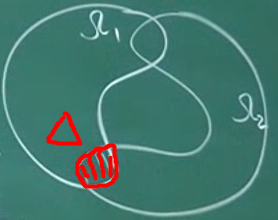
\includegraphics[width=5cm]{assets/04-functions-of-complex-variables/analitical-extension-difinition.png}
    \end{center}

    $f_2$ непосредственное аналитическое продолжение $f_1$ через $\Delta$, если $f_1(z) = f_2(z) \ \forall z \in \Delta$.
\end{definition}
\begin{remark}
    \begin{enumerate}
        \item {
            При фиксации $\Omega_1, \ \Omega_2, \Delta, f_1$, функция $f_2$ определена однозначно.

            \begin{proof}
                $g$ -- непоср. аналитическое продолжение $f_1$:

                $g(z) = f_1(z) = f_2(z) \ \forall z \in \Delta$

                $g, f_2 \in H(\Omega_2) \underbrace{\implies}_{\text{по т. единственности}} f_2 \equiv g$.
            \end{proof}
        }
        \item {
            Для другой компоненты продолжение может быть другим (тут понятнее на картинке, добавьте, плиз).
        }
    \end{enumerate}
\end{remark}

\begin{definition}
    $f \in H(\Omega), \ \tilde{f} \in H(\tilde{\Omega})$.

    $\tilde{f}$ -- аналитическое продолжение $f$ на цепочке областей, если $\exists \Omega_1, \dots \Omega_n$ и $f_1 \in H(\Omega_1), \dots , f_n \in H(\Omega_n)$, т.ч. $f_1$ -- непосредственное аналитическое продолжение $f$, $f_2$ -- непосредственное аналитическое продолжение $f_1, \dots, \tilde{f}$ -- непосредственное аналитическое продолжение $f_n$.
    % todo: picture

    \begin{center}
        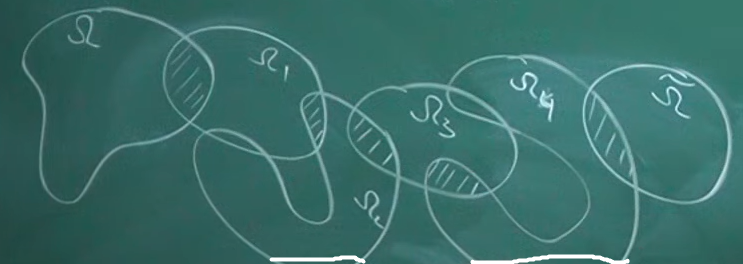
\includegraphics[width=11cm]{assets/04-functions-of-complex-variables/analitical-multiple-extension.png}
    \end{center}
\end{definition}



\begin{remark}
    Рассмотрим всевозможные пары $(f, \Omega)$, т.ч. $f \in H(\Omega)$, тогда существование аналитического продолжения по цепочке областей -- отношение эквивалентности на мн-ве таких пар.
\end{remark}


\begin{definition}
    Полная аналитическая функция -- класс эквивалентности.

    $F$ -- полная аналитическая ф-я. $M := \bigcup_{(f, \Omega) \in F} {\Omega}$ -- область определения (существования) $F$.
\end{definition}

\begin{statement}
    $M$ -- область.
\end{statement}
\begin{proof}
    \textbf{Открытость}: объединения открытых -- открытое.

    \textbf{Линейная связность}: $a, b \in M \implies a \in \Omega, b \in \tilde{\Omega}$. $(f, \Omega), \ (\tilde{f}, \tilde{\Omega})$ связана аналитическим продолжением по цепочке, будем переходить по соотвествующим областям и дойдем из $a$ в $b$.
\end{proof}


\begin{definition}
    $F$ -- полная аналитическая функция, $M$ -- область определения $F$, $z \in M$.

    $F(z) := \{ f(z): \ (f, \Omega) \in F \ \land \ z \in \Omega \}$.
\end{definition}

\begin{theorem}
    \textbf{Пуанкаре-Вольтерры}.

    $F(z)$ -- не более чем счетное мн-во.
\end{theorem}

\begin{example}
    $\underbrace{f(z)}_{\frac{1}{1-z}} = \sum_{n=0}^{\infty} {z^n}$ -- ряд сх-ся при $|z| < 1$

    % todo: picture.

    $\frac{1}{1 - z} = \frac{1}{(1-a) - (z - a)} = \frac{1}{1-a} \cdot \frac{1}{1 - \frac{z-a}{1-a}} = \frac{1}{1-a} \cdot \sum_{n=0}^{\infty} { \frac{(z-a)^n}{(1-a)^n} } = \sum_{n=0}^{\infty} { \frac{(z-a)^n}{(1-a)^{n+1}} }$

    $\left| \frac{z-a}{1-a} \right| < 1$ -- круг сходимости ряда.

    $|z-a| < |1-a|$

    % todo: picture
\end{example}


\begin{definition}
    $\sum_{n=0}^{\infty} { c_n \cdot (z - z_0)^n }$, $R$ -- радиус сх-ти ряда.

    % todo: picture

    Берем точку $w$ на границе круга ($|w - z_0| = R$). $w$ -- правильная точка, если найдется $U_w$ -- окр-ть точки $w$ и $g \in H(U_w)$ являющаяся непосредственным продолжением $f$.
\end{definition}

\begin{definition}
    Особая точка -- точка, не являющаяся правильной.
\end{definition}

\begin{theorem}
    На границе круга сх-ти лежит хотя бы одна особая точка.
\end{theorem}
\begin{proof}
    От противного.

    Пусть все точки правильные $|z| = R$ -- правильные.

    $f(z) = \sum_{n=0}^{\infty} { c_n z^n }, \ R$ -- радиус сх-ти.

    $\forall w: \ |w| = R$ -- правильная, тогда найдется $B_{r_w} (w)$ и $g \in H(B_{r_w} (w))$, т.ч. $f = g$ на пересечении $\{ |z| < R \} \cap \{ |z - w| < r_w \}$.

    То есть круги $B_{r_w}(w)$ покрывают окр-ть $|w| = R$. Это компакт, выберем конечное подпокрытие.

    % todo: picture

    По лемме Лебега $\exists \epsilon > 0: \ B_{\epsilon} (w)$ целиком содержится в элементе подпокрытия.

    $\{ |z| < R + \epsilon \} \subset \{ |z| < R \} \cup$ конечное подпокрытие.

    $h(z) := \begin{cases}
        f(z), \ |z| < R \\
        g_{w_j} (z), \ |z - w_j| < r_{w_j}
    \end{cases} \in H(\{ |z| < R + \epsilon \})$.

    % todo: picture
    $g(z) = \sum_{n=0}^{\infty} { c_n z^n }$ -- ряд Тейлора для $g$, он сх-ся в круге $|z| < R + \epsilon$.

    Противоречие тому, что радиус сходимости был $R$.
\end{proof}

\begin{example}
    \begin{enumerate}
        \item {
            $f(z) = \sum_{n=1}^{\infty} { \frac{z^n}{n^2} }$ сх-ся при $|z| \leq 1$.

            $f'(z) = \sum_{n=1}^{\infty} { \frac{z^{n-1}}{n} }$

            $(zf'(z))' = \sum_{n=0}^{\infty} { z^{n-1} } = \frac{1}{1-z}$
        }
        \item {
            $\sum_{n=0}^{\infty} { z^{2^n} }$ -- сх-ся при $|z| < 1$, все точки $|z| = 1$ -- особые.
            % todo: picture
        }
    \end{enumerate}
\end{example}


Начало 4-ого семестра.

% Начало 4 семестра
\begin{theorem}
    $f \in H(\Omega)$, \ $\Omega$ -- односвязная, $f \not = 0$ в $\Omega$.

    Тогда существует $g \in H(\Omega)$, т.ч. $e^{g(z)} = f(z)$ и $g$ -- единственна с точностью до аддит. константы $2 \pi i k, \ k \in \mathbb{Z}$.
\end{theorem}

\begin{proof}
    \textbf{Существование}:

    $\frac{f'}{f} \in H(\Omega) \implies $ есть первообразная $g \in H(\Omega)$.

    Подберем константу так, что $e^{g(z_0)} =  f(z_0)$ для некоторого $z_0 \in \Omega$.

    Покажем, что $g$ подходит: $h(z) := e^{-g(z)} \cdot f(z)$.

    Хотим доказать, что $h \equiv 1$. Знаем, что $h(z_0) = 1$ и

    $h'(z) = f'(z) e^{-g(z)} + f(z) e^{-g(z)} (-g'(z)) = e^{-g(z)} \left( f'(z) - f(z) \frac{f'(z)}{f(z)} \right) \equiv 0$.

    \textbf{Единственность}:

    Пусть $e^{g(z)} = f(z) = e^{\tilde{g}(z)} \implies e^{g(z) - \tilde{g}(z)} \equiv 1 \implies \underbrace{g(z) - \tilde{g}(z)}_{\in H(\Omega) \subset C(\Omega)} = 2 \pi i k_{z}: \ k_{z} \in \mathbb{Z} \implies g(z) - \tilde{g}(z) = 2 \pi i k$
\end{proof}

\begin{consequence}
    Пусть $0 \not \in \Omega$ -- односвязна, тогда существует единственный с точностью до $+ 2 \pi i k$ функция $g \in H(\Omega)$, т.ч. $e^{g(z)} = z$.
\end{consequence}

\begin{remark}
    $g(z) = \ln{|z|} + i \arg{z}$
\end{remark}

\begin{remark}
    Обозначение:

    $Ln(z) = \ln{|z|} + i Arg(z)$

    % todo: picture

    ветви логарифма
\end{remark}


\begin{properties}
    \begin{enumerate}
        \item $e^{Ln(z)} = z: \ \forall z \not = 0$
        \item $Ln(z w) = Ln(z) + Ln(w)$
        \item $Ln(z) = \ln{|z|} + i Arg(z)$, где $Arg(z) = \{ \arg{z} + 2 \pi i k: \ k \in \mathbb{Z} \}$
    \end{enumerate}
\end{properties}

\begin{remark}
    Св-во 2 для ветви может быть неверно.

    Берем конкретную ветку и точку:
    % todo: picture
    $0 < \arg < 2 \pi$

    $Ln(-i) = \underbrace{\ln{|-i|}}_{=0} + i Arg(-i) = \frac{3\pi i}{2}$

    $Ln((-i)^2) = Ln(-1) = \ln{|-1|} + i Arg(-1) = \pi i$

    Но $\pi i \not = \frac{3 \pi i}{2} + \frac{3 \pi i}{2}$
\end{remark}

\begin{remark}
    $z^p := e^{p Ln(z)}$ -- полная аналит. функция.

    Если $p \in \mathbb{Z}$, то все однозначно, т.к. $e^{p (2 \pi i k)} = 1$.

    Если $p \in \mathbb{Q}, \ p = \underbrace{\frac{m}{n}}_{\text{несократимая}}$, то $e^{\frac{m}{n} (2 \pi i k)}$ -- принимает $n$ значений.

    Если $p \in \mathbb{C} \setminus \mathbb{Q}$, то $e^{p (2 \pi i k)}$ -- принимает счетное кол-во значений.
\end{remark}



\begin{exerc}
    \begin{enumerate}
        \item Найти $i^i$
        \item Д-ть, что $(z^p)' = \frac{p z^p}{z}$ при $z \not = 0$
        \item $(z w)^p = z^p w^p$ как полные аналитичные функции, но это неверно для ветвей.
    \end{enumerate}
\end{exerc}


\Subsection{Ряды Лорана}

\begin{definition}
    $\sum_{n=-\infty}^{+\infty} a_n (z - z_0)^n$ -- ряд Лорана.

    $\sum_{n = 0}^{\infty} a_n (z - z_0)^n$ -- правильная часть.

    $\sum_{n = -\infty}^{-1} a_n (z - z_0)^n = \sum_{n = 1}^{\infty} a_{-n} (z - z_0)^{-n}$ -- главная часть.

    Ряд Лорана сходится $\Leftrightarrow$ правильная и главная части сходятся.

    Ниже будем считать, что $z_0 = 0$ для простоты записи.

    $\sum_{n=0}^{\infty} a_n z^n$ -- сх-ся в круге сх-ти $|z| < R$ -- радиус сх-ти $[0, +\infty]$.

    $\sum_{n = 1}^{\infty} a_{-n}z^{-n} = \sum_{n=1}^{\infty} a_{-n} w^{n}$, где $w = \frac{1}{z}$ -- сх-ся в круге сх-ти $|w| < \tilde{R} \implies |z| > \frac{1}{\tilde{R}} =: r$.

    То есть ряд Лорана сх-ся в кольце $r < |z| < R$ -- кольцо сх-ти ряда Лорана.
\end{definition}

\begin{properties}
    \begin{enumerate}
        \item Ряд Лорана абс. сх-ся в кольце $r < |z| < R$, где $r, R \in [0, +\infty]$
        \item В кольце, лежащем строго внутри кольца сх-ти, ряда Лорана сх-ся равномерно.
        \item В кольце сх-ти ряд Лорана можно почленно дифференцировать.
        \item Ряд Лорана в кольце сх-ти -- голоморфная функция.
    \end{enumerate}
\end{properties}

\begin{theorem}
    \textbf{О единственности ряда Лорана}.

    Пусть $f(z) = \sum_{n=-\infty}^{\infty} a_n z^n$ в кольце $r < |z| < R$.

    Тогда $a_n = \frac{1}{2 \pi i} \int_{|z| = \rho} {\frac{f(z)}{z^{n+1}} dz}$, где $r < \rho < R$.
\end{theorem}

\begin{proof}
    $\int_{|z| = \rho} { \frac{f(z)}{z^{n+1}} dz } = \int_{|z| = \rho} { \frac{\sum_{k = -\infty}^{+\infty} a_k z^k}{z^{n+1}} dz } =$

    $= \int_{|z| = \rho} { \sum_{k=-\infty}^{+\infty} a_k z^{k - n - 1} dz } = \sum_{k = -\infty}^{\infty} a_k \int_{|z| = \rho} { z^{k-n-1} dz } = 2\pi i a_n$ -- т.к. при $|z| = \rho$ ряд равномерно сходится, то можно интегрировать по-членно.

    $\int_{|z| = \rho} { z^m dz } = \int_{0}^{2\pi} { \rho^m e^{i m t} i \rho e^{i t} dt } = \rho^{m+1} i \int_{0}^{2\pi} { e^{i (m+1) t} dt } = \begin{cases}
        2 \pi i, \text{ при } m = -1 \\
        0, \text{ иначе}
    \end{cases}$
\end{proof}


\begin{remark}
    Нер-во Коши тут тоже выполняется:

    $|a_n| \leq \frac{M_{\rho}}{\rho^n}$, где $M_{\rho} = \max_{|z| = \rho}\{ |f(z)| \}$.
\end{remark}

\begin{theorem}
    \textbf{О существовании ряда Лорана}.

    Пусть $f \in H(r < |z| < R)$. Тогда $f(z) = \sum_{n = -\infty}^{+\infty} a_n z^n$, для некоторых $a_n \in \mathbb{C}$.
\end{theorem}
\begin{proof}
    $r < r_1 < r_2 < R_2 < R_1 < R$.

    \begin{center}
        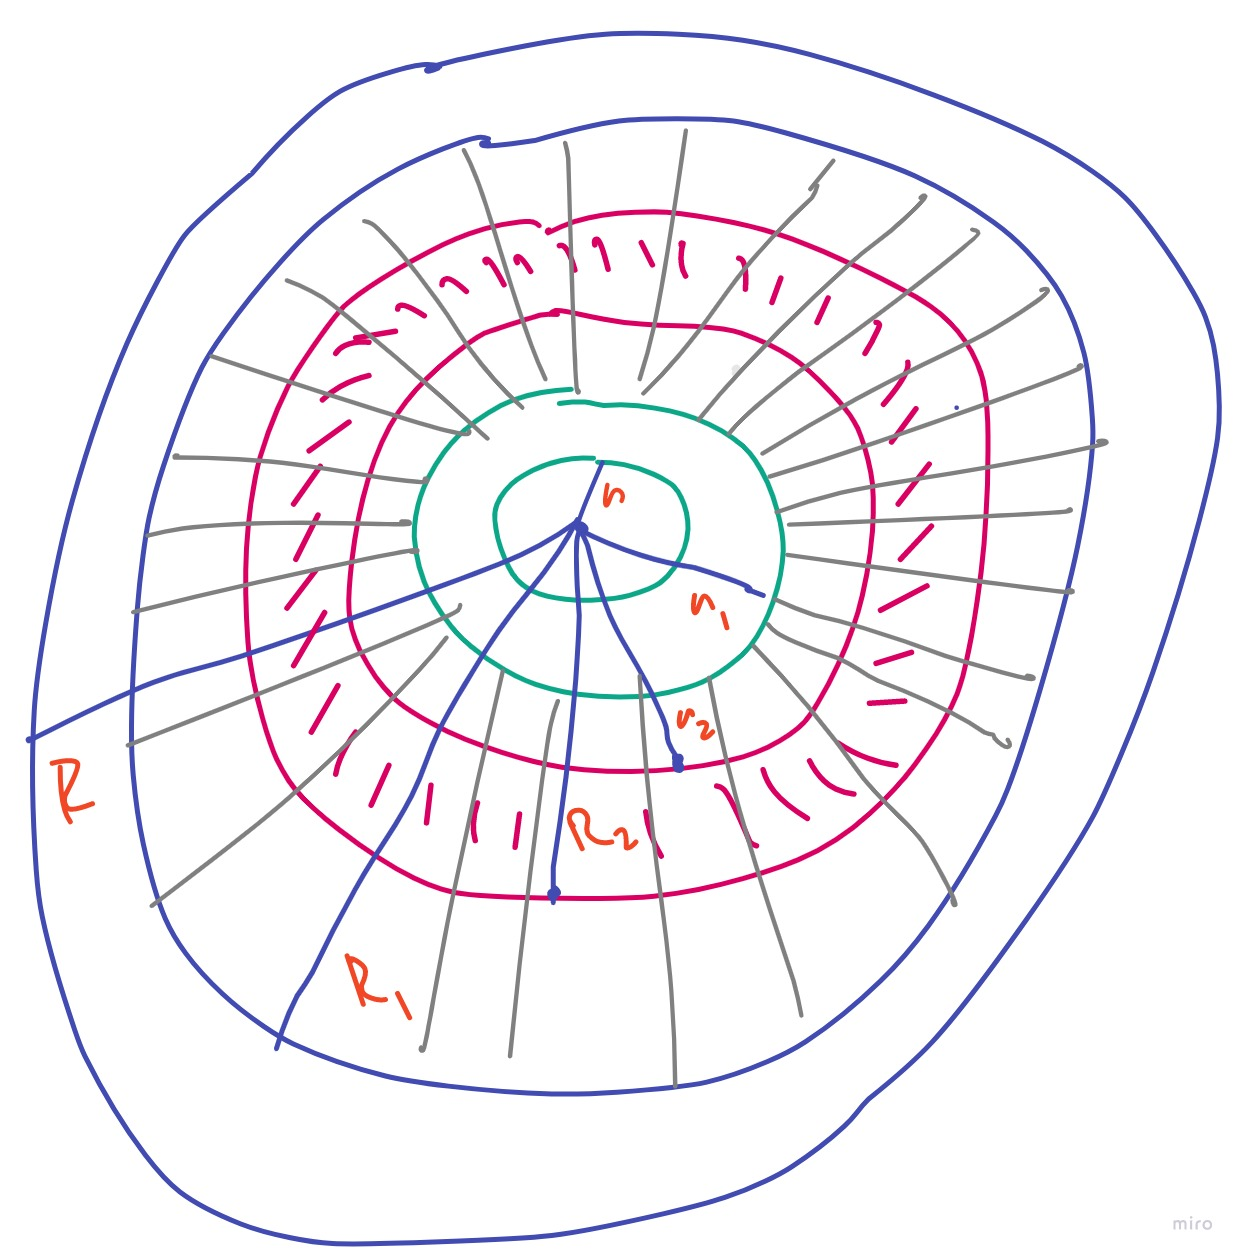
\includegraphics[height=6cm]{assets/04-functions-of-complex-variables/existence-of-function-decomposition-into-loran-series.jpg}
    \end{center}

    Берем $r_2 < |z| < R_2$: пишем для него и компакта $K =\{ r_1 \leq |z| \leq R_1 \}$ интегральную теорему Коши:

    $f(z) = \frac{1}{2 \pi i} \int_{\partial K} {\frac{f(\zeta)}{\zeta - z} d\zeta} = \frac{1}{2 \pi i} \int_{|\zeta| = R_1} { \frac{f(\zeta)}{\zeta - z} d\zeta } - \frac{1}{2 \pi i} \int_{|\zeta| = r_1} { \frac{f(\zeta)}{\zeta - z} d\zeta }$

    \begin{enumerate}
        \item {
            Пускай $|\zeta| = R_1, \ |z| < R_2, \ |\frac{z}{\zeta}| < \frac{R_2}{R_1} < 1$.

            Распишем: $\frac{1}{\zeta - z} = \frac{1}{1 - \frac{z}{\zeta}} \cdot \frac{1}{\zeta} = \sum_{n=0}^{\infty} { \frac{z^n}{\zeta^{n+1}} }$

            Считаем первое слагаемое:

            $\int_{|\zeta| = R_1} { \frac{f(\zeta)}{\zeta - z} d\zeta } = \int_{|\zeta| = R_1} { \sum_{n=0}^{\infty} z^n \frac{f(\zeta)}{\zeta^{n+1}} d\zeta } = \sum_{n = 0}^{\infty} {z^n \underbrace{\int_{|\zeta| = R_1} { \frac{f(\zeta)}{\zeta^{n + 1}} d\zeta }}_{=: a_n}}$ -- можем менять интеграл и сумму местами, из-за того, что ряд равномерно сходящийся.
        }
        \item {
            Теперь пускай $|\zeta| = r_1, \ |z| > r_2, \ |\frac{\zeta}{z}| < \frac{r_1}{r_2} < 1$.

            Распишем: $\frac{1}{\zeta - z} = -\frac{1}{z} \cdot \frac{1}{1 - \frac{\zeta}{z}} = -\sum_{n = 0}^{\infty} \frac{\zeta^n}{z^{n + 1}}$.

            Считаем второе слагаемое (переходы по аналогии):

            $-\int_{|\zeta| = r_1} { \frac{f(\zeta)}{\zeta - z} d\zeta } = \int_{|\zeta| = r_1} { \frac{1}{z^{n + 1}} f(\zeta) \zeta^n d\zeta } = \sum_{n=0}^{\infty} \frac{1}{z^{n+1}} \underbrace{\int_{|\zeta| = r_1}{f(\zeta) \zeta^n d\zeta}}_{=: a_{n-1}}$
        }
    \end{enumerate}

    Складывая воединино как раз и получим ряд Лорана для $f(z)$.
\end{proof}

\begin{theorem}
    Пусть $f \in H(r < |z| < R)$. Тогда существует $g \in H(|z| < R)$ и $h \in H(|z| > r)$, т.ч. $f(z) = g(z) + h(z)$. А если добавить условие: $h \rightarrow_{z \rightarrow \infty} 0$, то такое представление единственно.
\end{theorem}

\begin{proof}
    \textbf{Существование}:

    $f(z) = \sum_{n=-\infty}^{\infty} a_n z^n$.

    Пусть $g(z) = \sum_{n = 0}^{\infty}$ -- главная часть (сх-ся в $\{ |z| < R \}$), $h(z) = \sum_{n = -\infty}^{-1} a_n z^n$ -- правильная часть (сх-ся в $\{ |z| > r \}$).

    \textbf{Единственность}:

    Пусть $f(z) = g(z) + h(z)$, $f(z) = g_1(z) + h_1(z) \implies g(z) - g_1(z) = h_1(z) - h(z)$ при $r < |z| < R$.

    $F(z) := \begin{cases}
        g(z) - g_1(z), \text{ при } |z| < R \\
        h_1(z) - h(z), \text{ при } |z| > r
    \end{cases} \in H(\mathbb{C})$

    Поймем, что $F$ ограничена: $\lim_{z\rightarrow \infty} {F(z)} = 0 \implies$

    $|F(z)| \leq 1$ при $|z| \geq \rho$

    $|F(z)|$ -- огр. при $|z| \leq \rho$, так как $F(z)$ непрерывная на компакет.
    % по т. Вейерштрасса.

    Получили, что $F(z)$ голоморфна на $\mathbb{C}$ и ограничена $\implies_{\text{теорема Луивилля}}$ $F(z) \equiv const$.

    А так как $F(z) \rightarrow_{z \rightarrow +\infty} 0$, то $F(z) = 0 \implies g_1 = g_2$ и $h_1 = h_2$.
\end{proof}

\begin{definition}
    $a \in \mathbb{C}$. Если $f$ голоморфна в проколотой окрестности
    точки $a$, но не голоморфна в $a$, то $a$ - изолированная особая точка.

    $f \in H(0 < |z - a| < r)$
\end{definition}

\begin{definition}
    Если существует $\lim_{z \to a} f(z)$, то $a$ - устранимая особая точка.

    Если $\lim_{z \to a} f(z) = \infty$, то $a$ - полюс.

    Если $\lim_{z \to a}$ не существует, то $a$ существенно особая точка.
\end{definition}

\begin{example}
    \begin{enumerate}
        \item $\frac{\sin z}{z}, \frac{e^z - 1}{z}$. $z = 0$ - устранимая особая точка. Из Тейлора.
        \item $\frac{1}{z}, \frac{1}{\sin z}$. $z = 0$ - полюс.
        \item $e^{\frac{1}{z}}$. $z = 0$ - существенно особая точка. Предела нет, т.к. $\frac{1}{z_n} = 2\pi i n$, $\frac{1}{z_n} = 2\pi i n + \pi$. Разные последовательности точек.
    \end{enumerate}
\end{example}

\begin{theorem}
    \textbf{Характеристика устранимой особой точки}

    $f \in H(0 < |z - a| < r)$

    Следующие условия равносильны:
    \begin{enumerate}
        \item $a$ - устранимая особая точка
        \item $f$ ограничена в некоторой проколотой окрестности $a$
        \item $\exists \, g \in H(|z - a| < r)$, такая, что $f(z) = g(z) \forall \, z \neq a$
        \item В главной части ряда Лорана в точке $a$ все коэффициенты $0$
    \end{enumerate}
\end{theorem}

\begin{proof}
    \begin{enumerate}

        \item $4 \Rightarrow 3$ - очевидно
        \item $3 \Rightarrow 1$ - очевидно. $g$ непрерывна, предел $g(a)$
        \item $1 \Rightarrow 2$ - очевидно
        \item {
            Докажем $2 \Rightarrow 4$.

            Пусть ограничена $\forall \, 0 < |z - a| < r$: $f(z) \leqslant M$

            Запишем ряд Лорана: $f(z) = \sum_{n = -\infty}^{+\infty} c_n(z - a)^n$.

            Теперь воспользуемся нер-вом Коши для ряда Лорана: $|c_n| \leqslant \frac{\max |f(z)|}{\rho^n}$ при $|z - a| = \rho$.


            $c_{-n} \leqslant \rho^n \max f(z) \leqslant M \rho^n$ и устремим $\rho$ к $0$.

            Получаем, что $M \rho^n \rightarrow 0$, а тогда и $c_{-n} \rightarrow 0$.
        }
    \end{enumerate}
\end{proof}

\begin{theorem}
    \textbf{Характеристика полюса}

    Пусть $f \in H(0 < |z - a| < r)$

    Следующие условия равносильны:

    \begin{enumerate}
        \item $a$ -- полюс
        \item Существует $g \in H(|z - a| < r)$, $g(a) \neq 0$, такая, что $f(z) = \frac{g(z)}{(z - a)^m}, m \in \mathbb{N}$
        \item В главной части ряда Лорана в точке $a$ лишь конечное число ненулевых коэфцциентов. Но они есть.
    \end{enumerate}
\end{theorem}

\begin{proof}
    \begin{enumerate}
        \item {
            $2 \Rightarrow 3$:

            $g(z)$ -- голоморфна, тогда раскладывается по Тейлору:

            $g(z) = \sum_{n=0}^{\infty} c_n (z - a)^n, g(a) = c_0 \neq 0 \Rightarrow f(z) = \sum_{n = 0}^{+\infty} c_n(z - a)^{n - m}$ -- разложение в ряд Лорана, где $c^{-m} \neq 0$.
        }
        \item {
            $3 \Rightarrow 1$:

            $f(z) = \sum_{n = -m}^{\infty} b_n(z - a)^n$

            Все слагаемые $o((z - a)^{-m})$, тогда перепишем $f(z) = \sum_{n=-m}^{\infty} b_n \frac{(z-a)^{n + m}}{(z - a)^{m}}$ и становится видно, что при $z \rightarrow a$ каждая дробь стремится к $\infty$.

            % а на $b_{-m}(z - a)^{-m} \rightarrow \infty$
        }
        \item {
            $1 \Rightarrow 2$:

            $\lim_{z \to a} f(z) = \infty$

            Значит, в некоторой проколотой окрестности $0 <|z - a| < \varepsilon$:
            $|f(z)| > 1$.

            Рассмотрим $g(z) = \frac{1}{f(z)} \in H(0 < |z - a| < \varepsilon)$:

            $\lim_{z \to a} g(z) = 0$.

            Доопределим $g(a) = 0$ и получим $g \in H(|z - a| < \varepsilon)$.

            $a$ -- ноль функции $g$, тогда по теореме о нулях голоморфной функции $g(z) = (z - a)^m h(z)$, где $h(a) \neq 0$ и $h \in H(|z - a| < \varepsilon)$

            $\frac{1}{f(z)} = g(z) = (z - a)^m h(z)$, тогда $f(z) = (z - a)^{-m} \frac{1}{h(z)}$ и $\frac{1}{h(z)} \in H(|z - a| < \varepsilon)$, потому что $h$ не обращается в $0$.
        }
    \end{enumerate}
\end{proof}

\begin{definition}
    Это $m$ называется порядком полюса.
    \begin{remark}
        Это аналог кратности нуля
    \end{remark}
\end{definition}

\begin{remark}
    $f$ имеет в $a$ полюс порядка $m$ $\Longleftrightarrow \frac{1}{f}$ имеет в
    точке $a$ ноль кратности $m$ (доопределяем $\frac{1}{f}$ в $a$ пл непрерывности)

    А также $\Longleftrightarrow$ $f(z) = \sum_{n = -m}^{+\infty} c_n (z - a)^n$, где $c_m \neq 0$
\end{remark}

\begin{theorem}
    \textbf{Характеристика существенной особой точки}

    $f \in H(0 < |z - a| < r)$

    Следующие условия равносильны

    \begin{enumerate}
        \item $a$ - существенно особая точка
        \item В главной части ряда Лорана в точке $a$ бесконечное число ненулевых коэфф.
    \end{enumerate}
\end{theorem}

\begin{proof}
    Доказательство очевидно следует из предыдущего.
\end{proof}

\begin{definition}
    $f$ - мероморфная в $\Omega$, если $f \in H(\Omega \setminus E)$ и в точках из $E$ у неё полюсы
\end{definition}

\begin{example}
    $f = \ctg \frac{1}{z}$  - мероморфная в $\mathbb{C} \setminus 0$

    Полюсы в точках $z = \frac{1}{\pi k}$.

    Но при этом $\ctg \frac{1}{z}$ не будет мероморфной в $\mathbb{C}$. В точке $z = 0$ проблема.
    В любой окрестности 0, найдётся плохая точка, а значит она не изолированная особая.
\end{example}

\begin{remark}
    \begin{enumerate}
        \item $E$ не имеет предельных точек в $\Omega$.
        \item $E$ не более чем счётно.
    \end{enumerate}
\end{remark}

\begin{properties}
    Пусть $f$ и $g$ мероморфные в $\Omega$. Тогда:

    \begin{enumerate}
        \item {
            $f \pm g, \frac{f}{g}, fg, f'$ - мероморфны в $\Omega$.

            \begin{proof}

                Если подставляем точки, которые не полюсы и не нули, то голоморфность сохранится.

                Тогда пускай:

                $f(z) = \varphi (z) (z - a)^n$, $a$ -- полюс или $0$.

                $g(z) = \psi (z) (z - a)^m$, $a$ -- полюс или $0$.

                \begin{enumerate}
                    \item {
                        $fg$ и $\frac{f}{g}$:

                        Тогда $f(z)g(z) = (z - a)^{n + m} \underbrace{\varphi(z) \psi(z)}_{= (*)}$.

                        (*) -- в окр-ти точки $a$ голоморфна и в самой точке в ноль не обращается.

                        Для отношения по аналогии.
                    }
                    \item {
                        $f \pm g$:

                        Складываем ряды Лорана в точке $a$, в главной части $f \pm g$ конечное число ненулевых коэффициентов.
                    }
                    \item {
                        $f'$:

                        $f'(z) = (z - a)^n \varphi'(z) + n (z - a)^{n - 1} \varphi(z) = (z - a)^{n - 1} \cdot \underbrace{\left( (z - a) \varphi'(z) + n \varphi(z) \right)}_{= (*)}$

                        (*) -- в окр-ти точки $a$ голоморфна и в самой точке в ноль не обращается.

                        % $f'(z) = \varphi' (z) (z - a)^{-n} - n \varphi (z) (z - a)^{-n - 1} = (z - a)^{-n - 1}(z - a) - n\varphi (z) = \psi (z)$

                        % $\psi (z) = -n \varphi (a) \neq 0$
                    }
                \end{enumerate}
            \end{proof}
        }
        \item {
            Порядки полюсов у $f'$ на 1 больше, чем у $f$
        }
    \end{enumerate}
\end{properties}

\begin{statement}
    Если $f$ мероморфна в $\mathbb{C}$, то существует $g, h \in H(\mathbb{C})$, т.ч. $f = \frac{g}{h}$
\end{statement}

\begin{theorem}
    \textbf{Сохоцкого}

    Пусть $a$ - существенно особая точка функции $f$. Тогда $Cl \left(f(0 < |z - a| < \varepsilon)\right) = \mathbb{C} \cup \{ \infty \}$

    Более того, $\forall b \in \mathbb{C} \cup \{ \infty \}$ найдётся такая последовательность
    $z_n \rightarrow a$, т.ч. $f(z_n) \rightarrow b$
\end{theorem}

\begin{proof}
    \begin{enumerate}
        \item Случай $b = \infty$. $f$ не ограничена в $0 < |z - a| < \frac{1}{n}$. Иначе $a$ была бы устранимой особой точкой.
        Значит найдётся $z_n$, такое что $0 < |z_n - a| < \frac{1}{n}$ и $|f(z_n)| \geqslant n$.
        $z_n \rightarrow a$ и $f(z_n) \rightarrow \infty$
        \item $b \in \mathbb{C}$. Если найдётся последовательность $z_n \rightarrow a$, т.ч. $f(z_n) = b$, то всё ясно.
        Если не найдётся, то в некоторой проколотой окретности $0 < |z - a| < \varepsilon $ $f(z) \neq b$
        Тогда рассмотрим $g(z) = \frac{1}{f(z) - b} \in H(0 < |z - a| < \varepsilon)$.
        $a$ - изолированнная особая точка для $g$.

        $f(z) = b + \frac{1}{g(z)}$

        Если $a$ - полюс у $g$, то $a$ - устранимая особая точка $f$ - не подходит

        Если $a$ - устранимая особая точка $g$, то $a$ - устранимая особая точка $f$ или полюс - не подходит

        Значит $a$ - существенно особая точка $g$. Воспользуемся уже доказанным случаем для $g$.
        Найдётся $z_n \rightarrow a$, такая, что $g(z_n) \rightarrow \infty$. А тогда
        $\lim f(z_n) = b$.
    \end{enumerate}
\end{proof}

\begin{theorem}
    \textbf{Пикара}

    Пусть $a$ - существенно особая точка $f$ и $\varepsilon > 0$. Тогда
    $f(0 < |z - a| < \varepsilon) = \mathbb{C}$ или $\mathbb{C}$ без одной точки.
\end{theorem}

\begin{example}
    $f(z) = e^{\frac{1}{z}}$ не обращается в ноль, хотя $z = 0$ - существенно особая точка.
\end{example}

\begin{definition}
    Бексонечные пределы. $\lim z_n = \infty \Longleftrightarrow \lim |z_n| = +\infty$
\end{definition}

\begin{properties}

    \item Если $\lim z_n = \infty$, $w_n$ ограничена. Тогда $\lim (z_n \pm w_n) = \infty$
    \item $\lim z_n = 0 \Longleftrightarrow \lim \frac{1}{z_n} = \infty$
    \item Если $\lim z_n = \infty$ и $|w_n| \geqslant c > 0$, то $\lim z_nw_n = \infty$

    Доказательства очевидны + с первого курса
\end{properties}

\begin{definition}
    $f \in H(|z| > R)$. $f$ голоморфна в $\infty$, если там устранимая особая точка. То есть $\lim_{z \to \infty} f(z) \in \mathbb{C}$

    \begin{remark}
        $g(z) = f(\frac{1}{z}) \in H(0 < |z| < \frac{1}{R})$ - перешли от бесконечности к нулю.
    \end{remark}
\end{definition}

\begin{remark}
    $f \in H(|z| > R), g(z) = f(\frac{1}{z}) \in H(0 < |z| < \frac{1}{R})$
    \begin{enumerate}
        \item $\infty$ - устранимая особая точка $f \Longleftrightarrow 0$ - устранимая особая точка $g$
        \item $\infty$ - полюс $f \Longleftrightarrow 0$ - полюс $g$
        \item $\infty$ - существенно особая точка $f \Longleftrightarrow 0$ - существенно особая точка $g$

        $f(z) = \sum_{n = -\infty}^{+\infty} c_nz_n, g(z) \sum_{n = -\infty}^{+\infty}$
        \item $\infty$ - устранимая особая точка $f \Longleftrightarrow$ коэфф. при положительных степенях $0$
        \item $\infty$ - полюс $f \Longleftrightarrow$ при положительных степенях лишь конечное число ненулевых коэфцциентов.
        \item $\infty$ - существенно особая точка $f \Longleftrightarrow$ при положительных степенях беск. число ненулевых коэфф.
    \end{enumerate}
\end{remark}

\begin{theorem}
    \textbf{Луивилля}

    Если $f \in H(\bar{\mathbb{C}})$, то $f \equiv const$
\end{theorem}

\begin{proof}
    $\lim_{z \to \infty} f(z) \in \mathbb{C}$, значит при больших ограничена. $|f(z)| \leqslant M$ для $|z| > R$.
    С другой стороны $f \in C(|z| \leqslant R)$. Значит $|f(z)| \leqslant \bar{M}$.
    По теореме Лиувилля(старой), $f \equiv const$
\end{proof}

\newpage

\begin{definition}
    \textbf{Стереографическая проекция}
    \begin{center}
        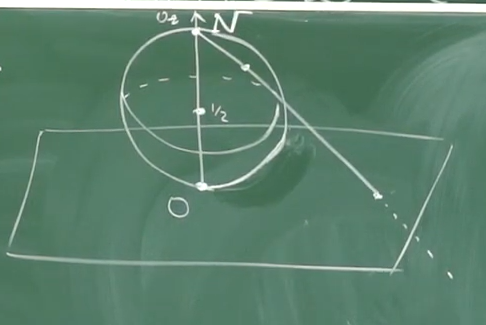
\includegraphics{assets/04-functions-of-complex-variables/stereo-graphical-projection.png}
    \end{center}

    $z = x + iy$ - плоскость. $(u, v, w) \in \mathbb{R}^3$.

    $u^2 + v^2 + (w - \frac{1}{2})^2 = \frac{1}{2^2}$

    Или же $u^2 + v^2 + w^2 = w$ - уравнение сферы Римана.
\end{definition}

\begin{theorem}
    \textbf{Связь между точкой на плоскости и точной на сфере}

    Точке $z$ соответсвует точка с координатами $(\frac{x}{1 + |z|^2}, \frac{y}{1 + |z|^2}, \frac{|z|^2}{1 + |z|^2})$

    \begin{remark}
        Точке $(u, v, w)$ соответсвует точка $z = x + iy = \frac{u}{1 - w} + i \frac{v}{1 - w}$
    \end{remark}
\end{theorem}

\begin{proof}
    Прямая через точки $(0, 0, 1)$ и $(x, y, 0)$. Параметризация луча:
    $(xt, yt, 1 - t)$. Нас интересует точка, в которой луч пересекает сферу, то есть:

    $(xt)^2 + (yt)^2 + (1- t)^2 = 1 - t$.

    $(x^2 + y^2 + 1)t^2 + 1 - 2t = 1 - t \Leftrightarrow t = \frac{1}{x^2 + y^2 + 1} = \frac{1}{|z|^2 + 1}$
\end{proof}

\begin{consequence}
    \begin{enumerate}
        \item Расстояние между образами $z$ и $\tilde{z}$ равно $\rho = \frac{|z - \tilde{z}|}{\sqrt{1 + |z|^2} \cdot \sqrt{1 + |\tilde{z}|^2}}$,
        а расстояние между $z$ и $\infty$ равно $\frac{1}{\sqrt{1 + |z|^2}}$

        \textbf{Доказательство:} предложено посчитать самому, у кого есть силы добавьте, плиз.

        \item Сходимость на плоскости и сходимость на сфере Римана совпадают

        \textbf{Доказательство:} $z_n \to z_0 \Rightarrow \frac{|z_n - z_0|}{\sqrt{1 + |z_n|^2}\cdot \sqrt{1 + |z_0|^2}} \to 0$

        $z_n \to \infty \Leftrightarrow \frac{1}{\sqrt{1 + |z_n|^2}} \to 0$

        Пусть $\frac{|z_n - z_0|}{\sqrt{1 + |z_n|^2}\cdot \sqrt{1 + |z_0|^2}} \to 0$

        Тогда $\frac{|z_n - z_0|}{\sqrt{1 + |z_n|^2}} \to 0$. Если $z_n$  ограничена, то $|z_n - z_0| \to 0$

        Если не ограничена, то возьмём $|z_{n_k}| \to \infty$, тогда $\frac{|z_{n_k} - z_0|}{\sqrt{1 + |z_{n_k}|^2}} \to 1$

        \item $\mathbb{C} \cup \{ \infty \}$ - компакт.
    \end{enumerate}
\end{consequence}

\Subsection{Вычеты}

\begin{definition}
    $a$ - изолированная особая точка. $f \in H(0 < |z - a| < R)$.
    $f(z) = \sum_{n = -\infty}^{+\infty} c_n (z - a)^n$ - сходится при $0 < |z - a| < R$.

    $\res_{z = a} f = c_{-1}$
\end{definition}

\begin{definition}
    $f \in H(|z| > R)$ раскладывается в $f(z) = \sum_{n = -\infty}^{+\infty} c_n z^n$

    $\res_{z = \infty} f(z) = -c_{-1}$
\end{definition}

\begin{properties}
    \begin{enumerate}
        \item $f \in H(0 < |z - a| < R)$ и $0 < r < R$.

        Тогда $\res_{z = a} f = \frac{1}{2\pi i} \int_{|z - a| = r} f(z) \, dz$ - положительный обход
        точки $a$.

        \textbf{Доказательство:} смотреть формулу для коэффициентов ряда Лорана.

        \item $f \in H(|z| > R), r > R$.

        Тогда $\res_{z = \infty} f = -\frac{1}{2\pi i} \int_{|z| = r} f(z) \, dz = \frac{1}{2\pi i} \int_{|z| = r} f(z) \, dz$ -
        положительный обход для $\infty$

        \item Если $a \in \mathbb{C}$ - полюс $n$-го порядка.

        Тогда $\res_{z = a} f(z) = \lim_{z \to a} \frac{1}{(n - 1)!} \frac{d^{n - 1}}{dz^{n - 1}} ((z - a)^n f(z))$

        \textbf{Доказательство:} Считаем, что $a = 0$.

        $f(z) = \sum_{k = -n}^{+\infty} c_kz^k \Rightarrow g(z) = z^n f(z) = \sum_{k = 0}^{\infty} c_{k - n}z^k $ - формула Тейлора.

        Тогда $c_{-1} = \frac{g^{(n - 1)}(0)}{(n - 1)!}$.

        \item Если $a \in \mathbb{C}$ - полюс первого порядка.

        Тогда $\res_{z = a} f(z) = \lim_{z \to a} (z - a)f(z)$

        \item Если $a \in \mathbb{C}$, $g$ и $h$ голоморфны в окрестности точки $a$.
        $h(a) = 0, h'(a) \neq 0, g(a) \neq 0$. $f(z) = \frac{g(z)}{h(z)}$

        Тогда $\res_{z = a} f(z) = \frac{g(a)}{h'(a)}$

        \textbf{Доказательство:} $\res_{z = a} f(z) = \lim_{z \to a} (z - a)f(z) =
        \lim_{z \to a} \frac{z - a}{h(z) - h(a)} g(z) = \frac{g(a)}{h'(a)}$

        \item Если $\lim_{z \to \infty} f(z) = A \in \mathbb{C}$.

        Тогда $\res_{z = \infty} f(z) = \lim_{z \to \infty} z (A - f(z))$

        \textbf{Доказательство:} $f(z) = A + \sum_{k = -\infty}^{-1} c_nz^n$, правильная часть - константа,
        иначе всё бы пошло на бесконечность.

        \item $\res_{z = \infty} f(z) = -\res_{z = 0} \frac{f(\frac{1}{z})}{z^2}$

        \textbf{Доказательство:} $f(z) = \sum_{n = -\infty}^{\infty} c_nz^n$

        $\frac{1}{z^2} f(\frac{1}{z}) = \frac{1}{z^2} \sum_{n = -\infty}^{\infty} c_nz^{-n} =
        \sum_{n = -\infty}^{\infty} c_nz^{-n - 2}$
    \end{enumerate}
\end{properties}

\begin{theorem}
    \textbf{Коши о вычетах}

    $f$ голоморфна в $\Omega$, за исключением точек $a_1, \ldots a_n$.
    $K \subset \Omega$ - компакт и $a_1 \ldots a_n \in Int K$

    Тогда $\int_{\partial K} f(z) \, dz = 2\pi i \sum_{k = 1}^n \res_{z = a_k} f(z)$
\end{theorem}

\begin{proof}

    У каждой точки можем взять окрестность, чтобы они лежали внутри компакта и
    попарно не пересекаются. $\widetilde{K} = K \setminus \bigcup_{k = 1}^n B_{\varepsilon} (a_k)$ - компакт.

    А ещё $f \in H(\Omega \setminus \{ a_1 \ldots a_n\} )$

    Из интегральной формулы Коши: $\int_{\partial \widetilde{K}} f(z) \, dz = 0$

    Но $\int_{\partial \widetilde{K}} f(z) \, dz = \int_{\partial K} f(z) \, dz - \sum_{k = 1}^n \int_{|z - a_k| = \varepsilon} f(z) \, dz$, а
    под знаком суммы - вычеты.


    \begin{center}
        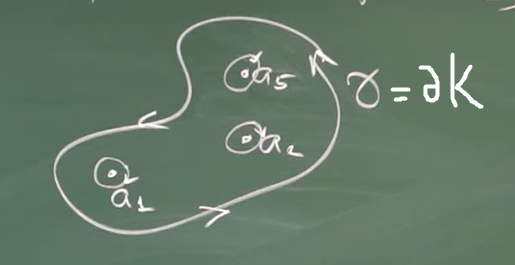
\includegraphics{assets/04-functions-of-complex-variables/koshi-theorem-for-deductions.png}
    \end{center}
\end{proof}

\begin{consequence}
    Если $f$ голоморфна в $\mathbb{C} \setminus \{ a_1 \ldots a_n \} $, то
    $\res_{z = \infty} f(z) + \sum_{k = 1}^n \res_{z = a_k} f(z) = 0$

    \textbf{Доказательство:} возьмём круг $B_R (0)$, внутри которого содержатся все эти точки.

    $\int_{|z| = R} f(z) \, dz = 2 \pi i \sum_{j = 1}^n \res_{z = a_j} f(z)$.

    Но также $\int_{|z| = R} f(z) \, dz = \int_{|z| = R}{ \sum_{k = -\infty}^{\infty} c_k z^k dz } = -2 \pi i \res_{z = \infty} f(z)$. Перекидываем и доказываем.
\end{consequence}

\begin{example}
    \begin{enumerate}
        \item {
            $\int_{|z| = 4} \frac{z^4}{e^z + 1} \, dz = 2 \pi i (\res_{z = \pi i} + \res_{z = -\pi i}) = -4\pi^5 i$.

            Особые точки: $e^z = -1$ при $z = \pi i + 2 \pi i k$.

            Пусть $g(z) = z^4, h(z) = e^z + 1 \implies f = \frac{g}{h}$.

            $\pi i$ -- полюс первого порядка: $\res_{z = \pi i} f = \frac{g(\pi i)}{h'(\pi i)} = -\pi^4$

            $-\pi i$ -- полюс первого порядка: $\res_{z = -\pi i} f = \frac{g(-\pi i)}{h'(-\pi i)} = -\pi^4$
        }
        \item {
            $\int_{-\infty}^{\infty} \frac{dx}{1 + x^{2n}} = \lim_{R \to +\infty} \int_{-R}^{R} \frac{dx}{1 + x^{2n}}$.

            \begin{center}
                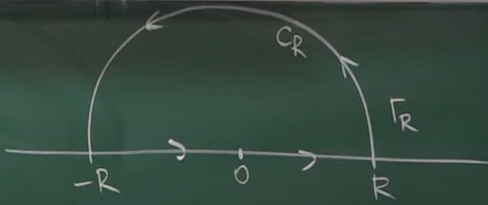
\includegraphics[width=12cm]{assets/04-functions-of-complex-variables/example-2-cauchy-about-deductions.png}
            \end{center}

            Контур - полукруг. $I := \int_{\Gamma_R} \frac{dz}{1 + z^{2n}} = 2 \pi i \sum \res$

            Но с другой стороны $\int_{\Gamma_R} = \int_{-R}^R + \int_{c_R}$

            $| \int_{c_R} \frac{dz}{1 + z^{2n}}| \leqslant \underbrace{\pi R}_{\text{длина кривой}} \cdot \underbrace{\max \left|\frac{1}{1 + z^{2n}}\right|}_{\text{макс. подъинтегрального выражения}} = \pi R \frac{1}{\min |1 + z^{2n}|}
            \underbrace{\leqslant}_{|a + b| \geqslant |a| - |b|} \frac{\pi R}{R^{2n} - 1} \rightarrow_{R \to \infty} 0$

            Значит то, что мы хотим найти - просто сумма вычетов.

            Какие особые точки?

            $z^{2n} = -1 \implies z = e^{\frac{\pi i k}{2n}}$ и $k$ нечётно.

            Нас интересует $k = 1, 3 \ldots 2n - 1$

            Тогда $I = 2 \pi i \sum_{k = 1}^n \res_{2k - 1}$

            Все $a_k$ -- полюсы первого порядка:

            (*): так как все $a_k$ - корни уравнения $z^{2n} = -1$, то $a_k^{2n} = -1$.

            $\res_{a_k} f = \frac{1}{(z^{2n} + 1)'} \big|_{z = a_k} = \frac{1}{2n \cdot a_k^{2n - 1}} = \frac{a_k}{2n\cdot a_k^{2n}} \underbrace{=}_{(*)} -\frac{a_k}{2n}$.
        }
        \item {
            Оптимизация решения из предыдущего пункта: мы хотим считать не по всей дуге, а по какой-то ее части (до такого угла $\alpha$, что интеграл $\int_{R\cdot e^{i\alpha}}^{0}$ был бы равен исходному интегралу, домноженному на какую-то константу).

            $\int_{-\infty}^{+\infty} \frac{dx}{1 + x^{2n}} = 2\int_{0}^{+\infty} \frac{dx}{1 + x^{2n}} = I$ - т.к. функция $f(z) = \frac{1}{1 + x^{2n}}$ четная.

            \begin{center}
                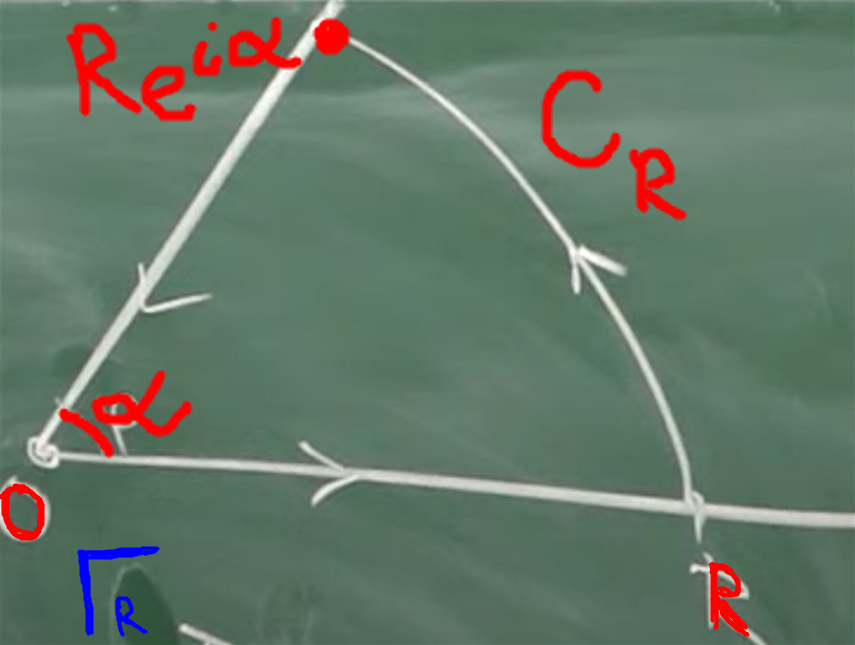
\includegraphics[width=12cm]{assets/04-functions-of-complex-variables/example-3-cauchy-about-deductions.png}
            \end{center}

            $f(x) = \frac{1}{1 + z^{2n}}$.

            $\int_{\Gamma_R} f(z) \, dz = \int_{c_R} + \int_{0}^{R} + \int_{Re^{i\alpha}}^{0}$ - интеграл по контуру разбили на кусочки.

            $\int_{R \cdot e^{i\alpha}}^{0} f(z) \, dz = -\int_{0}^{R \cdot e^{i \alpha}} \underbrace{=}_{z=e^{i\alpha} \cdot t, \ t \in [0, R]} -\int_{0}^{R} f(e^{i \alpha} t) e^{i \alpha} \, dt$ -
            взяли параметризацию $z \to e^{i \alpha} t$.

            $f(e^{i \alpha}t) = \frac{1}{1 + e^{2n\cdot i\cdot \alpha} \cdot t^{2n}} \underbrace{=}_{\text{Хотим: } e^{2n\cdot i\cdot \alpha} = 1} \frac{1}{1 + t^{2n}}$, $\alpha = \frac{\pi}{n}$.

            Единственная особая точка $e^{\frac{i \pi}{2n}}$ (т.к. особые точки имеют вид $e^{\frac{\pi i k}{2n}}$, и мы хотим, чтобы точка лежала \textbf{строго внутри контура}: $0 < \frac{\pi k}{2n} < \alpha \Rightarrow 0 < \frac{\pi k}{2n} < \frac{\pi}{n} \Rightarrow k=1$).

            Тогда, так как особая точка для контура $\Gamma_{R}$ всего одна, то интеграл $\int_{\Gamma_{R}}$ равен: $2 \pi i \res_{z=e^{\frac{i \pi}{2n}}}$.

            Получаем равенство (при этом $\int_{C_R} \rightarrow 0$, т.к. он еще меньше того, что мы считали выше, поэтому про $\int_{C_R}$ можно забыть): $2 \pi i \res_{z=e^{\frac{i \pi}{2n}}} = \int_{\Gamma_{R}} = I - e^{i\frac{\pi}{n}}\cdot I + \int_{C_R} \implies$

            $\implies I - e^{i \frac{\pi }{n}} I = 2 \pi i \res_{z = e^{\frac{i \pi}{2n}}} f = 2 \pi i \cdot \left ( - \frac{e^{\frac{i \pi}{2n}}}{2n}  \right )$ - вычет именно такой, так как наша точка является полюсом 1-ого порядка, следовательно применимо свойство вычета $f(z) = \frac{g(z)}{h(z)} \Rightarrow res_{z=a}f = \frac{g(a)}{h'(a)}$.

            Тогда $I = -\frac{2 i e^{\frac{i \pi}{2n}}}{1 - e^{\frac{i \pi}{2n}}} \cdot \frac{\pi}{2n} = \frac{2 i \cdot e^{\frac{2 \pi}{2n}}}{e^{\frac{i \pi}{2n}} \cdot (e^{\frac{i \pi}{2n}} - e^{-\frac{i \pi}{2n}})} \cdot \frac{\pi}{2n} = \frac{\pi}{2n \cdot \sin \frac{\pi}{2n}}$ - т.к. $\sin(z) = \frac{e^{iz} - e^{-iz}}{2i}$
        }
    \end{enumerate}
\end{example}

\begin{lemma}
    \textbf{Жордана}

    $C_{n} = \{ z \in \mathbb{C} : |z| = R_n, \Im z \geqslant 0 \}$, $R_n \rightarrow +\infty$

    $g : \{ \Im z \geqslant 0 \} \to \mathbb{C}$

    $M_{n} = \sup_{z \in C_{n}} |g(z)| \rightarrow_{n \to \infty} 0$

    Тогда $\forall \, \lambda > 0 \, : \, \int_{C_{n}} g(z) e^{i \lambda z} \, dz \rightarrow_{n \to \infty} 0$
\end{lemma}

\begin{proof}
    Пусть $f(z) = g(z) e^{i \lambda z}$.

    \begin{center}
        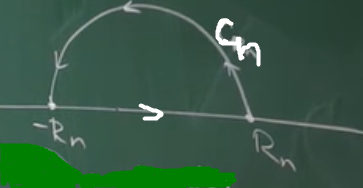
\includegraphics[width=7cm]{./assets/04-functions-of-complex-variables/Jordan's-lemma-proof.png}
    \end{center}

    Введем параметризацию: $z = R_n e^{i t}, \ dz = R_n e^{it} i dt$, где $t \in [0, \ \pi]$, тогда получим

    $\int_{C_{n}} f(z) dz = i \int_{0}^{\pi} R_n e^{it} \cdot f\left(R_n e^{it}\right) dt$

    Оценим этот интеграл по модулю:

    $\left| i \int_{0}^{\pi} R_n e^{it} f\left(R_n e^{it}\right) dt \right| \leq R_n \int_{0}^{\pi} \underbrace{\left| g\left(R_n e^{it}\right) \right|}_{\leq M_{n}} \cdot \left| e^{i \lambda R_n e^{it}} \right| dt \leq M_n R_n \int_{0}^{\pi} \cdot \left| e^{i \lambda R_n e^{it}} \right| dt = (*)$


    Поймем, что такое $|e^{i \lambda R_n e^{it}}|$:

    $Re\left( i \lambda R_n e^{it} \right) = \lambda R_n Re\left(i e^{it}\right) = \lambda R_n (-\sin{t})$

    Тогда можем продолжить оценивать исходный интеграл, но предварительно заметим, что под интегралом записана выражение симметричное относительно $\frac{\pi}{2}$, тогда переписываем так:

    $(*) = 2 M_n R_n \int_{0}^{\frac{\pi}{2}} e^{-\lambda R_n \sin{t}} dt \underbrace{\leq}_{(**)} 2 M_n R_n \int_{0}^{\frac{\pi}{2}} e^{-\lambda R_n \frac{2}{\pi} t} dt = 2 M_n R_n \frac{1 - e^{-\lambda R_n}}{\lambda R_n \frac{2}{\pi}} \leq \frac{\pi M_n}{\lambda} \rightarrow_{n \to \infty} 0$.

    $(**)$: верно, так как при $0 \leq t \leq \frac{\pi}{2}: \ \sin(t) \geq \frac{2}{\pi} t$.
\end{proof}

\begin{example}
    $\int_0^{+\infty} \frac{\cos x}{1 + x^2} \, dx = I$.

    Можем считать на всей прямой и не исходный интеграл, а $\int_{-\infty}^{+\infty} \frac{e^{ix}}{1 + x^2} = I^*$.

    Тогда $\Re I^* = 2I$.

    \begin{center}
        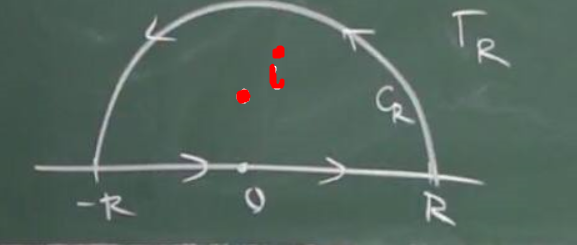
\includegraphics[width=7cm]{./assets/04-functions-of-complex-variables/example-for-jordan-lemma.png}
    \end{center}

    Пусть $f(z) = \frac{e^{iz}}{1 + z^2}$.

    Контур - полуокружность от $-R$ до $R$.

    $\int_{\Gamma_R} f(z) \, dz = \int_{-R}^{R} + \int_{C_R}$.

    Здесь $\int_{C_R} \rightarrow 0$ по лемме Жордана, где $\lambda = 1$ и $M_R = \sup_{|z| = R} \left | \frac{1}{1 + z^2} \right | \leqslant \frac{1}{R^2 - 1} \rightarrow 0$

    (написанное выше верно, так как $|1 + z^2| \geqslant |z^2| - 1 = R^2 - 1$)

    Тогда $\int_{\Gamma_R} f(z) \, dz = 2 \pi i \sum \res f = 2 \pi i \cdot \res_{z = i} f = (*)$.

    $i$ - полюс 1-ого порядка, тогда $f(z) = \frac{g(z)}{h(z)}$, где $g(i) \neq 0, h(i) = 0, h'(i) \neq 0$:

    $\res_{z=i} f = \frac{g(i)}{h'(i)} = \frac{e^{-1}}{2i}$.

    Тогда $(*) = \frac{\pi}{e} \implies I = \frac{\pi}{2e}$

\end{example}

\begin{lemma}
    \textbf{О полувычете}

    $f \in H(0 < |z - a| < R)$ и $a$ - полюс первого порядка. $C_{\varepsilon} = \{ z \in \mathbb{C} : |z - a| = \varepsilon, \alpha \leqslant \arg (z) \leqslant b \}$

    \begin{center}
        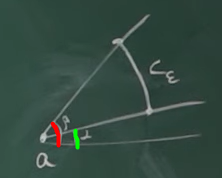
\includegraphics[width=9cm]{assets/04-functions-of-complex-variables/lemma-about-half-deduction.png}
    \end{center}

    Тогда $\lim_{\varepsilon \to 0+} \int_{C_{\varepsilon}} f(z) \, dz = (\beta - \alpha) i \cdot \res_{z = a} f$
\end{lemma}

\begin{proof}
    Считаем, что $a = 0$.
    
    У нас полюс 1-го порядка, тогда $f(z) = \frac{c}{z} + g(z)$, где $g \in H(|z| < R)$.

    Параметризация $z = \varepsilon e^{it}$, где $t \in [\alpha, \beta]$. Тогда $dz = \varepsilon e^{it} i \, dt$.

    $\int_{C_{\varepsilon}} f(z) \, dz = \int_{C_{\varepsilon}} \frac{c}{z} \, dz + \int_{C_{\varepsilon}} g(z) \, dz =
    \int_{\alpha}^{\beta} \frac{c}{\varepsilon e^{it}} \cdot \varepsilon e^{it} i \, dt + \int_{C_{\varepsilon}} g(z) \, dz = (\beta - \alpha) \cdot i \cdot c + \int_{C_{\varepsilon}} g(z) \, dz$

    Оценим второй интеграл:

    $g$ -- голоморфма, тогда ограничена в окр. точки $\implies |g| \leq M$.
    
    $\left|\int_{C_{\varepsilon}} g(z) \, dz\right| \leqslant M \underbrace{\varepsilon (\beta - \alpha)}_{\text{длина дуги}}$, где $M = \max_{|z| \leqslant \frac{R}{2}} |g(z)|$. и
    тогда $\int_{C_{\varepsilon}} g(z) \, dz \rightarrow 0$.
\end{proof}

\begin{definition}
    \textbf{Главное значение интеграла} ($v.p. \int$).

    $\int_{a}^{b} f(x) \, dx$, где $c$ - единственная особая (в этой точке нет непрерывности функции) точка, $c \in (a, b)$.

    $\int_{a}^{c - \varepsilon} f(x) \, dx + \int_{c + \varepsilon}^{b} f(x) \, dx$
    и устремляем $\varepsilon$ к нулю. Предел - главное значение интеграла.
\end{definition}

\begin{example}
    $v.p. \int_{-1}^{1} \frac{dx}{x} = 0$.

    $\lim_{\varepsilon \rightarrow 0+} \int_{-1}^{-\varepsilon} + \int_{\varepsilon}^{1} = 0$, потому что
    фукнция нечетная.

    $v.p. \int_{-\infty}^{\infty} \frac{dx}{x} = 0$
\end{example}

\begin{properties}
    \begin{enumerate}
        \item {
            Если $\int$ сходится, то $\int = v.p. \int$
        }
        \item {
            Линейность
        }
        \item {
            Аддитивность, если резать не по особым точкам
        }
    \end{enumerate}
\end{properties}

\begin{example}
    $I = \int_{0}^{+\infty} \frac{\sin x}{x} \, dx$

    Функция четная, поэтому $2I = \int_{-\infty}^{+\infty} \frac{\sin x}{x} \, dx = v.p. \int_{-\infty}^{+\infty} \frac{\sin x}{x} \, dx$

    ($\frac{e^{ix}}{x} = \frac{1}{x} + \frac{ix}{x} + \ldots$).

    Тогда $2I = \Im v.p. \int_{-\infty}^{+\infty} \frac{e^{ix}}{x} \, dx$

    $v.p. \int_{-\infty}^{+\infty} = \lim_{\varepsilon \to 0, R \to +\infty} \int_{-R}^{-\varepsilon} + \int_{\varepsilon}^{R}$.

    \begin{center}
        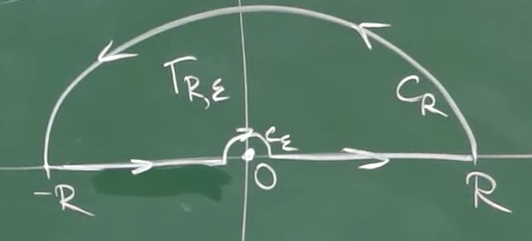
\includegraphics[width=8cm]{assets/04-functions-of-complex-variables/example-principal-value-integral.png}
    \end{center}

    $f(z) = \frac{e^{iz}}{z}$

    $\int_{\Gamma_{R, \varepsilon}} f(z) \, dz = 0$, так как особая точка только $0$, а она не в контуре.

    Но с другой стороны: $\int_{\Gamma_{R, \varepsilon}} f(z) \, dz = \int_{-R}^{-\varepsilon} + \int_{\varepsilon}^{R} + \int_{C_R} + \int_{C_{\varepsilon}}$

    \begin{enumerate}
        \item {
            $\int_{-R}^{-\varepsilon} + \int_{\varepsilon}^{R} \rightarrow v.p. \int_{-R}^{R}$
        }
        \item {
            $\int_{C_R} \rightarrow 0$ -- по лемме Жордана.
        }
        \item {
            $\int_{C_{\varepsilon}} f(z) \, dz \rightarrow -\pi i \cdot res_{z = 0} f = (-\pi i)$ -- лемма о полувычете, где $\alpha=\pi$, $\beta=0$, $0$ -- полюс 1-го порядка.
        }
    \end{enumerate}

    
    А значит $v.p. \int_{-\infty}^{\infty} \frac{e^{ix}}{x} \, dx = \pi i$.
    
    Тогда $I = \frac{1}{2} \Im \left(v.p. \int_{-\infty}^{\infty} \frac{e^{ix}}{x} \, dx\right) = \frac{\pi}{2}$
\end{example}

\newpage

\begin{example}
    $I = \int_{0}^{+\infty} \frac{x^{p - 1}}{1 + x} \, dx $, где $0 < p < 1$.

    \begin{center}
        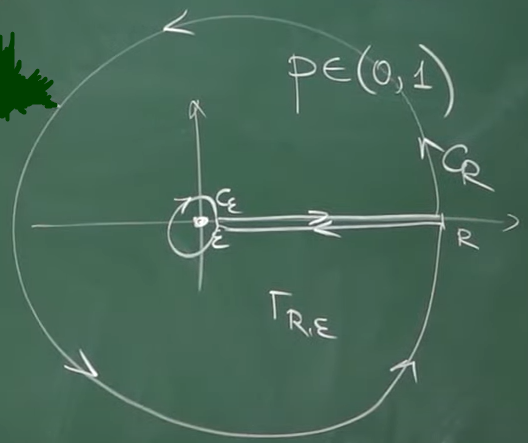
\includegraphics[width=7cm]{assets/04-functions-of-complex-variables/example-2-principal-value-integral.png}
    \end{center}

    $f(z) = \frac{e^{(p - 1) Ln z}}{1 + z}$, и пусть $Ln (1) = 0$.

    $\int_{\Gamma_{R, \varepsilon}} f(z) \, dz = \int_{\varepsilon}^{R} + \int_{Re^{2\pi i}}^{\varepsilon e^{2\pi i}} + \int_{C_{\varepsilon}} + \int_{C_R}$.

    Но с другой стороны $\int_{\Gamma_{R, \varepsilon}} f(z) \, dz = 2 \pi i \sum \res f = 2 \pi i \res_{z = -1} f$

    $\res_{z = -1} f = e^{(p - 1) Ln (-1)} = e^{(p - 1)\pi i} = -e^{p \pi i}$

    \begin{enumerate}
        \item {
            $\int_{\varepsilon}^{R} \rightarrow I$
        }
        \item {
            $\int_{Re^{2\pi i}}^{\varepsilon e^{2 \pi i}} = \int_{R}^{\varepsilon} \frac{e^{(p-1)\cdot (ln(x) + 2\pi i)}}{1 + x}dx = e^{2\pi i \cdot (p-1)} \cdot (-1)\cdot \int_{\varepsilon}^{R} \frac{x^{p - 1}}{1 + x} dx \rightarrow -e^{(p - 1) 2 \pi i} \cdot I = -e^{2\pi p i} \cdot I$
        }
        \item {
            $\left | \int_{C_{R}} \frac{e^{(p - 1)Ln z}}{1 + z} \, dz \right | \leqslant 2\pi R \cdot \max_{|z| = R} \left | \frac{e^{(p - 1) Ln z}}{1 + z} \right | =
            2\pi R \cdot \frac{R^{p - 1}}{\min |1 + z|} = 2\pi R \cdot \frac{R^{p - 1}}{R - 1} \rightarrow 0$

        }
        \item {
            $\left | \int_{C_{\varepsilon}} \frac{e^{(p - 1)Ln z}}{1 + z} \, dz \right | \leqslant 2\pi \varepsilon \cdot \max_{|z| = \varepsilon} \left | \frac{e^{(p - 1) Ln z}}{1 + z} \right | =
            2\pi \varepsilon \cdot \frac{\varepsilon^{p - 1}}{\min |1 + z|} = 2\pi \varepsilon \cdot \frac{\varepsilon^{p - 1}}{1 - \varepsilon} \rightarrow 0$
        }

        Тогда получаем, что $I - e^{2 \pi p i} \cdot I = -2 \pi i e^{\pi p i} \implies$
        
        $\implies I = \frac{2 \pi i e^{\pi p i}}{e^{2 \pi p i} - 1} = \pi \cdot \frac{2 i}{e^{\pi p i} -e^{-\pi p i}} = \frac{\pi}{\sin {(\pi p)}}$.
    \end{enumerate}
\end{example}

\begin{theorem}

    Пусть $f$ - мероморфная функция в $\mathbb{C}$. $z_1, \ldots, z_n$ - полюсы.
    $G_1, \ldots, G_n$ - главные части рядов Лорана в точках $z_1, \ldots, z_n$.
    $\infty$ - полюс или устранимая особая точка. $G$ - правильная часть
    ряда Лорана в $\infty$

    Тогда $f(z) = G(z) + \sum_{k = 1}^n G_k(z) + C$, в частности,
    $f$ - рациональная функция.
\end{theorem}

\begin{proof}
    $g(z) = f(z) - G(z) - \sum_{k = 1}^n G_k(z)$. У этой функции $z_1, \ldots, z_n, \infty$ -
    устранимые особые точки, а во всех остальных точках есть голоморфность.

    Тогда по теореме Луивилля $g \equiv const$.
\end{proof}

\begin{theorem}
    Пусть $f$ мероморфная функция в $\mathbb{C}$, $z_1, z_2 \ldots$ -- полюсы,
    $R_1, R_2, \ldots$ -- последовательность радиусов, т.ч. $R_n$ возрастают и $R_n \rightarrow +\infty$, $M_{R_n} = \max_{|z| = R_n} |f(z)| \rightarrow 0$.

    Тогда $f(z) = \lim_{n \to \infty} \sum_{k:|z_k| < R_n} G_k (z)$.
\end{theorem}

\begin{proof}
    $I_n(z) := \frac{1}{2\pi i}\int_{|\zeta| = R_n} {\underbrace{\frac{f(\zeta)}{\zeta - z}}_{=: g(\zeta)} d\zeta} = \sum res \ g = res_{\zeta = z} \ g(\zeta) + \sum_{k : \ |z_k| < R_n} res_{\zeta = z_k} \ g$

    \begin{enumerate}
        \item {
            $res_{\zeta = z} \ g = \frac{f(\zeta)}{(\zeta - z)'}|_{\zeta = z} = f(z)$ -- формула для полюса $1$-ого порядка.
        }
        \item {
            $res_{\zeta = z_k} \ g = \underbrace{res_{\zeta = z_k} \ \frac{f(\zeta) - G_k(\zeta)}{\zeta - z}}_{\text{голоморфна в окр. $z_k$, т.е. равна $0$}} + res_{\zeta = z_k} \ \frac{G_k(\zeta)}{\zeta - z}$

            Рассмотрим окр. радиуса $R$ и запишем интеграл $\frac{1}{2 \pi i} \int_{|\zeta| = R} {\frac{G_k(\zeta)}{\zeta - z} d\zeta} = res_{\zeta = z} \ \frac{G_k(\zeta)}{\zeta - z} + res_{\zeta = z_k} \ \frac{G_k(\zeta)}{\zeta - z}$ -- так как все особые точки для подъинтегрального выражения это $z$ и $z_k$.


            $res_{\zeta = z} \ \frac{G_k(\zeta)}{\zeta - z} = G_k(z)$ (по формуле для полюса 1-ого порядка), а второе слагаемое равно тому, что мы хотим найти.

            $\left| \int_{|\zeta| = R} {\frac{G_k(\zeta)}{\zeta - z} d\zeta} \right| \leq 2\pi R \cdot \frac{O\left(\frac{1}{R}\right)}{R - |z|} \rightarrow_{R \to \infty} 0$, где $G_k = \frac{c_{-1}}{\zeta - z_k} + \frac{c_{-2}}{(\zeta - z_k)^2} + \ldots = O(\frac{1}{R})$ (кол-ва слагаемых конечно, т.к. $a_k$ -- полюс).

            Из стремления к нулю, мы поняли, что $res_{\zeta = z_k} \ \frac{G_k(\zeta)}{\zeta - z} = -G_k(z)$.
        }
    \end{enumerate}


    Теперь мы имеем, что $I_n(z) = f(z) - \sum_{k: \ |z_k| < R_n} G_k(z)$, осталось доказать, что $\lim_{n \rightarrow \infty} I_n(z) = 0$.

    Вспоминаем, что  $I_n(z) := \frac{1}{2\pi i}\int_{|\zeta| = R_n} {\frac{f(\zeta)}{\zeta - z} d\zeta}$ и тогда:

    $\left| I_n(z) \right| \leq \frac{1}{2 \pi} \cdot 2\pi R_n \cdot max_{|\zeta| = R_n} \left| \frac{f(\zeta)}{\zeta - z} \right| \leq R_n \cdot \frac{M_{R_n}}{R_n - |z|} \rightarrow_{n \to \infty} 0$.

    % $\frac{1}{2\pi i} \int_{|\zeta| = R_n} \frac{f(\zeta)}{\zeta - z} \, d \zeta = \sum \res \frac{f(\zeta)}{\zeta - z} = (*)$

    % $\left| \frac{1}{2\pi i} \int_{|\zeta| = R_n} \frac{f(\zeta)}{\zeta - z} \, d \zeta \right| = R_n \cdot
    % \max_{|\zeta| = R_n} \left | \frac{f(\zeta)}{\zeta - z} \right | \leqslant R_n \cdot \frac{M_{R_n}}{R_n - |z|} \rightarrow 0$

    % Какие особые точки есть у $(*)$ -- особые точки $z$ и особые точки $f$.
    % Поймём, как устроены вычеты в этих особых точках.

    % \begin{enumerate}
    %     \item {
    %         $\res_{\zeta = z} \frac{f(\zeta)}{\zeta - k}$ - полюс первого порядка, значит:

    %         $\res_{\zeta = z} \frac{f(\zeta)}{\zeta - k} = f(z)$
    %     }
    %     \item {
    %         $\res_{\zeta = z_k} \frac{f(\zeta)}{\zeta - z} = \res_{\zeta = z_k} \frac{G_k (\zeta)}{\zeta - z}$, так как разность -- голоморфная в точке $z_k$ функция.

    %         Такой вычет посчитаем так, посчитаем интеграл по кружности радиуса $R$:

    %         $\frac{1}{2\pi i} \int_{|\zeta| = R} \frac{G_k (\zeta)}{\zeta - z} \, d\zeta = \res_{\zeta = z} + \res_{\zeta = z_k}$.

    %         С другой стороны:

    %         $\left | \frac{1}{2\pi i} \int_{|\zeta| = R} \frac{G_k (\zeta)}{\zeta - z} \, d\zeta \right | \leqslant R \cdot \frac{\max_{|\zeta| = R} |G_k (\zeta)|}{R - |z|} \rightarrow 0$.

    %         А значит $-\res_{\zeta = z} = \res_{\zeta = z_k}$.

    %         Отсюда получили, что $\res_{\zeta = z_k} \frac{G_k (\zeta)}{\zeta - z} = \res_{\zeta = z} \frac{G_k(\zeta)}{\zeta - z} = -G_k (z)$.
    %     }
    % \end{enumerate}
    % Тогда $(*) = f(z) - \sum_{k : |z_k| < R_n} G_k (z)$.
\end{proof}

% \begin{example}
%     $f(z) = \frac{\ctg z}{z}$. Особые точки вида $\pi k, k \in \mathbb{Z}$. Давайте брать $R_n = \pi n + \frac{\pi}{2}$.

%     % Тут, наверное, нужна картинка.

%     \begin{lemma}
        % Существует $M$, такая что, $|\ctg z| \leqslant M$ при $|z| = \pi (n + \frac{1}{2})$.
%     \end{lemma}

%     $M_{R_n} \leqslant \frac{M}{R_n} \rightarrow 0$. Тогда исходя из теоремы
%     $\frac{\ctg z}{z} = \lim_{n \to \infty} \sum_{-n}^n G_k(z)$, где $G_k$ - главная часть ряда Лорана в точке
%     $\pi k$.

%     Пусть $k \neq 0$, тогда $f$ имеет в точке $\pi k$ полюс первого порядка.
%     Тогда $G_k(z) = \frac{\res}{z - \pi k}$.

%     Нас интересует $\res_{z = \pi k} \frac{\ctg z}{z} = \res_{z = \pi k} \frac{\frac{\cos z}{z}}{\sin z}$.
%     Числитель и знаменатель голоморфны и $z = \pi k$ - ноль первой кратности. Тогда
%     $\res = \frac{\frac{\cos z}{z}}{(\sin z)'} = \frac{1}{\pi k}$.

%     Поэтому $G_k(z) = \frac{1}{\pi k(z - \pi k)}$

%     $z = 0$. Интересуемся $G_0(z) = \frac{a}{z} + \frac{b}{z^2}$. Здесь $a = 0$, так как функция чётная, $b =
%     \res_{z = 0} \ctg z = \res_{z = 0} \frac{\cos z}{\sin z} = 1$.

%     То есть $\frac{\ctg z}{z} = \frac{1}{z^2} \lim_{n \to \infty} \sum_{k = 1}^n \left ( \frac{1}{\pi k(z - \pi k)} - \frac{1}{\pi k(z + \pi k)} \right ) =
%     \frac{1}{z^2} + \sum_{k = 1}^{\infty} \frac{2}{z^2 - \pi^2 k^2}$

%     \begin{proof}
%         \textbf{леммы про $\ctg$}

%         Нужен рисунок, без него беда. Тут потеряно доказательство.
%         %Рисунок и пруф.
%     \end{proof}
% \end{example}

\begin{example}
    $\ctg(z) = \frac{1}{z} + \sum_{k=1}^{\infty} \frac{2z}{z^2 - \pi^2 k^2}$
\end{example}

\begin{lemma}
    Существует $M$, такая что, $|\ctg z| \leqslant M$ на окружностях $|z| = \pi (n + \frac{1}{2})$, где $n \in \mathbb{N}$.
\end{lemma}
\begin{proof}
    Леммы.

    Наблюдения про $\ctg z$:
    \begin{enumerate}
        \item $\pi$-периодическая функция $\implies$ все значения содержатся в полосе $0 \leq Re(z) \leq \pi$, можно все окружности сдвинуть по периоду.
        \item нечетная функция $\implies$ можем интересоваться только половиной картинки (давайте смотреть на $Re(z) \geq 0$).
    \end{enumerate}

    \begin{center}
        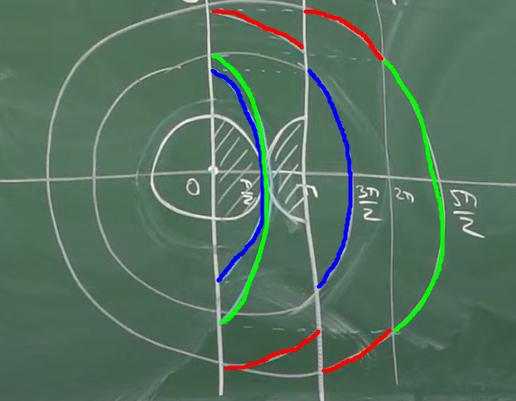
\includegraphics[width=9cm]{assets/04-functions-of-complex-variables/ctg-lemma.png}
    \end{center}

    Мы получаем полосу, за некоторым исключением (так как есть определенные точки, которые точно не получаются):

    $\{ 0 \leq Re(z) \leq \pi \} \setminus \{ |z| < \frac{\pi}{2} \} \cup \{ |z - \pi| < \frac{\pi}{2} \}$.

    Получаем следующее мн-во:

    \begin{center}
        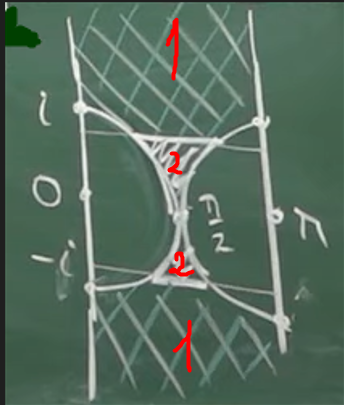
\includegraphics[height=6cm]{assets/04-functions-of-complex-variables/ctg-lemma-2.png}
    \end{center}

    Хотим понять, что $\ctg$ ограничен на заштриховоном мн-ве.

    $z = x + iy$

    \begin{enumerate}
        \item {
            Зона 1 ($y \geq 1$ или $y \leq -1$, в силу нечетности $\ctg$):

            $|\ctg z| = |\frac{\cos z}{\sin z}| = \left|\frac{e^{iz} + e^{-iz}}{e^{iz} - e^{-iz}}\right| = \left| \frac{1 + e^{2iz}}{1 - e^{2iz}} \right| \leq  \frac{1 + \left|e^{2iz}\right|}{\left|1 - e^{2iz}\right|} = (*)$

            Пусть $z = x + iy$ и пока что $y \geq 1$:

            $|e^{2iz}| = |e^{2ix} \cdot e^{-2y}| = e^{-2y}$, тогда $(*) = \frac{1 + e^{-2y}}{|1 - e^{2iz}|} \leq \frac{1 + e^{-2y}}{1-e^{-2y}} \leq \frac{2}{1 - e^{-2}}$
        }
        \item {
            Зона 2:

            Очевидно, что эта зона это компакт, а $\ctg$ на ней непрерывен $\implies$ $\ctg$ -- ограничен на этом компакте.
        }
    \end{enumerate}
\end{proof}

\begin{proof}
    Примера.

    $f(z) = \frac{\ctg z}{z}$, из леммы: $\ctg z \leq M$ при $|z| = \pi (n + \frac{1}{2})$.

    Берем радиусы $R_n = \pi (n + \frac{1}{2}) \implies M_{R_n} \leq \frac{M}{\pi (n + \frac{1}{2})} \rightarrow 0$.

    Особые точки $f(z): \ z = 0 \text{ -- полюс 2-ого порядка}, z = \pi k \text{ -- полюсы 1-ого порядка при } k \neq 0$.

    $G_k$ -- главная часть ряда Лорана в $\pi k, \ k \neq 0$ $\implies G_k(z) = \frac{res_{z = \pi k} \ \frac{\ctg(z)}{z}}{z - \pi k} = \frac{1}{\pi k(z - \pi k)}$, где $res_{z = \pi k} \ \frac{\ctg(z)}{z} = \frac{\frac{\cos(z)}{z}}{\sin'(z)} |_{z = \pi k} = \frac{1}{\pi k}$.


    $G_0(z) = \frac{A}{z^2} + \frac{res_{z = 0} \ f(z)}{z} = \frac{A}{z^2}$, вычет занулился, так как $f(z)$ -- четная функция и все коэффициенты перед нечетными степенями в ряде Лорана равны $0$.

    $G_0(z) = \frac{A}{z^2} = \frac{1}{z^2}$, так как $\frac{\ctg(z)}{z} = \frac{\cos(z)}{z \sin(z)} \sim \frac{1}{z^2}$ при $z$ близких к нулю.

    То есть $\frac{\ctg(z)}{z} = G_0(z) + \sum_{k=1}^{\infty} \left(G_{k}(z) + G_{-k}(z)\right) =$

    $= \frac{1}{z^2} + \sum_{k=1}^{\infty} \left( \frac{1}{\pi k(z - \pi k)} + \frac{1}{\pi (-k) (z + \pi k)} \right) = \frac{1}{z^2} + \sum_{k=1}^{\infty} \frac{2}{z^2 - \pi^2 k^2}$.
\end{proof}

\begin{example}
    $(\ln \sin z)' = \ctg z$

    $(\ln \frac{\sin z}{z})' = \ctg z - \frac{1}{z}$.

    $\ln \frac{\sin z}{z} = \int_{0}^{z} (\ctg w - \frac{1}{w}) \, dw = \int_{0}^{z} \sum_{k=1}^{\infty} \frac{2w}{w^2 - \pi^2 k^2} \, dw =
    \sum_{k = 1}^{\infty} \int_{0}^{z} {\frac{2w}{w^2 - \pi^2 k^2} dw}$ (можем переставлять, потому что есть равномерная сходимость).

    $\sum_{k = 1}^{\infty} \int_{0}^{z} \left ( \frac{1}{w - \pi k} + \frac{1}{w + \pi k} \right ) =$

    $= \sum_{k = 1}^{\infty} \ln (w - \pi k) + \ln (w + \pi k) \bigg |_{0}^z = \sum_{k = 1}^{\infty} \ln
    \left ( \frac{z^2 - \pi^2 k^2}{-\pi^2 k^2} \right ) = \sum_{k = 1}^{\infty} \ln \left ( 1 - \frac{z^2}{\pi^2 k^2} \right )$.

    Тогда $\frac{\sin z}{z} = \prod_{k = 1}^{\infty} \left(1 - \frac{z^2}{\pi^2 k^2} \right)$.

    Либо $\sin z = z \prod_{k = 1}^{\infty} \left(1 - \frac{z^2}{\pi^2 k^2} \right)$.
\end{example}

\begin{example}
    $\sum_{n = 1}^{\infty} \frac{1}{n^2} = \frac{\pi^2}{6}$

    $f(z) = \frac{1}{z^2}$. Посмотрим на $f(z) \cdot \ctg (\pi z)$. Тогда
    $\res_{z = k} f(z) \cdot \ctg (\pi z) \underbrace{=}_{f(k)\neq 0} \frac{f(z)\cdot \cos{\pi z}}{(\sin{\pi z})'}|_{z=k}  = \frac{f(k)}{\pi}$ - т.е. если $f(k) \neq 0$, то $z=0$ - полюс кратности 1, значит $\res_{z=a}f = \frac{g(a)}{h'(a)}$ при условии, что $f(z) = \frac{g(z)}{h(z)}$.

    $g(z) = \frac{\ctg \pi z}{z^2}$ и проинтегрируем.

    $\frac{1}{2 \pi i} \int_{|z| = n + \frac{1}{2}} \frac{\ctg \pi z}{z^2} \, dz =
    \sum_{k = -n, k \neq 0}^n \frac{1}{\pi k^2} + \res_{z = 0} \frac{\ctg \pi z}{z^2}$.

    При этом есть такая оценка:
    $\left | \frac{1}{2 \pi i} \int_{|z| = n + \frac{1}{2}} \frac{\ctg \pi z}{z^2} \, dz \right | \leqslant
    (n + \frac{1}{2}) \cdot \frac{M}{(n + \frac{1}{2})^2} \rightarrow 0$

    Значит, $\sum_{k = 1}^{\infty} \frac{1}{k^2} = -\frac{\pi}{2} \cdot \res_{z = 0} \frac{\ctg \pi z}{z^2}$.

    Такой вычет не очень приятно считать -- раскладываем в ряд (хотим найти коэфф $c_{-1}$ перед $\frac{1}{z}$, т.к. это и есть вычет по определению). Тогда нужно найти коэфф. перед $z^1$ в разложении $\ctg{z}$, т.к. потом мы поделим на $\frac{1}{z^2}$ и получим то, что надо.

    (*): $\frac{1}{1-t} = 1 + t + o(t), \ t \rightarrow 0$

    Найдем коэффициент перед $z^1$: в разложении $\ctg \pi z = \frac{\cos \pi z}{\sin \pi z} = \frac{1 - \frac{\pi^2 z^2}{2} + \mathcal{O}(z^4)}{\pi z (1 - \frac{\pi^2 z^2}{6} + \mathcal{O}(z^4))} \underbrace{=}_{(*)} $


    $ = \frac{(1 - \frac{\pi^2 z^2}{2} + \mathcal{O}(z^4))(1 + \frac{\pi^2 z^2}{6} + \mathcal{O}(z^4))}{\pi z} = \frac{1}{\pi z} - \frac{1}{3} \pi z + \mathcal{O}(z^3)$.

    То есть этот коэффициент равен: $-\frac{\pi}{3}$.

    Тогда $\sum_{k = 1}^{\infty} \frac{1}{k^2} = -\frac{\pi}{2} \cdot (-\frac{\pi}{3}) = \frac{\pi^2}{6}$.
\end{example}

\begin{theorem} (О числе нулей и полюсов).

    Пусть $f$ мероморфна в $\Omega$, $\gamma$ - простая замкнутая кривая в $\Omega$,
    не проходящая через нули и полюсы $f$.

    Тогда $\frac{1}{2 \pi i} \int_{\gamma} \frac{f'(z)}{f(z)} \, dz = \mathcal{N}_f - \mathcal{P}_f$

    $\mathcal{N}_f$ - количество нулей $f$ с учетом кратности в контуре $\gamma$.

    $\mathcal{P}_f$ - количество полюсов $f$ с учетом кратности (порядка) в контуре $\gamma$.

    \begin{consequence}
        Если $f \in H(\Omega)$, $\gamma$ - простая замкнутая кривая, не проходящая через нули $f$, тогда
        $\frac{1}{2\pi i} \int_{\gamma} \frac{f'(z)}{f(z)} \, dz = \mathcal{N}_f$
    \end{consequence}
\end{theorem}

\begin{proof} Теоремы.

    Если $a$ - ноль или полюс $f$, то $f(z) = (z - a)^m g(z)$, где $g(a) \neq 0$ и
    $g$ голоморфна в окрестности $a$.

    \begin{enumerate}
        \item Если $a$ - ноль, то $m$ - кратность нуля
        \item Если $a$ - полюс, то $m$ - порядок полюса.
    \end{enumerate}

    $f'(z) = m(z - a)^{m - 1} g(z) + (z - a)^m g'(z)$

    $\frac{f'(z)}{f(z)} = \frac{m}{z - a} + \frac{g'(z)}{g(z)}$, второе слагаемое голоморфно в окрестности $a$. Значит,
    $a$ - полюс первого порядка $\frac{f'}{f}$, а $m$ - вычет.
\end{proof}

\begin{consequence}
    \textbf{Принцип аргумента}

    Пусть $f \in H(\Omega)$, $\gamma$ - простая замкнутая кривая в $\Omega$, не проходящая через
    нули $f$.

    Тогда $\mathcal{N}_f = \frac{1}{2\pi} \Delta_{\gamma} \arg f(z)$, где $\Delta_{\gamma}$ - изменение аргумента
    при движении по кривой.
\end{consequence}

\begin{proof}
    $\mathcal{N}_f = \frac{1}{2\pi i} \int_{\gamma} \frac{f'(z)}{f(z)} \, dz$. Но $\frac{f'}{f} = (Ln f)'$.
    Если рассмотрим $Ln$ на кривой $\gamma$, то это будет первообразная вдоль пути $\gamma$ для $\frac{f'}{f}$.

    $\mathcal{N}_f = \frac{1}{2\pi i} \Delta_\gamma (Ln f(z)) = \frac{1}{2 \pi i} (\Delta_\gamma
    (\ln |f(z)| + i\arg f(z))) = \frac{1}{2\pi} \Delta_{\gamma} \arg f(z)$
\end{proof}

\begin{theorem}
    \textbf{Руше}

    $f, g \in H(\Omega)$, $\gamma$ - простой замкнутая кривая в $\Omega$ и
    $|f| > |g|$ на $\gamma$.

    Тогда $f + g$ и $f$ внутри $\gamma$ имеют одинаковое число нулей с учетом кратности.
\end{theorem}

\begin{proof}
    $\mathcal{N}_{f + g} = \frac{1}{2 \pi} \Delta_\gamma \arg (f + g)$.
    $|f + g| \geqslant |f| - |g| > 0$ на $\gamma$, поэтому в ноль обращения нет и
    можно использовать принцип аргумента.

    $\mathcal{N}_{f + g} = \frac{1}{2\pi} \Delta_\gamma \arg (f \cdot (1 + \frac{g}{f})) =
    \frac{1}{2\pi} \Delta_\gamma \arg f + \frac{1}{2\pi} \Delta_\gamma \arg (1 + \frac{g}{f})$.

    Значит надо доказать, что $\Delta_\gamma \arg (1 + \frac{g}{f}) = 0$.

    Значения $1 + \frac{g}{f}$ на $\gamma$ лежат в круге $|z - 1| < 1$, потому что $\frac{|g|}{|f|} < 1$. А значит
    вокруг нуля обойти не можем и изменения аргумента нет.
\end{proof}

\begin{example}
    $z - e^{-z} = \lambda > 1$. Хотим понять, что в правой полуплоскости есть ровно 1 корень.

    \begin{center}
        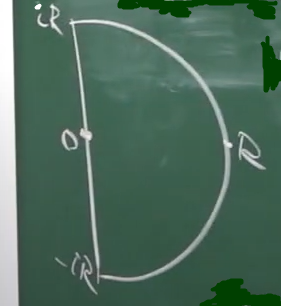
\includegraphics[width=7cm]{assets/04-functions-of-complex-variables/rushe-example.png}
    \end{center}

    Возьмём окружность большого радиуса и по ней обход по контуру $\gamma$.

    Возьмём $f(z) = z - \lambda$ и $g(z) = -e^{-z}$. Хотим подставить в т. Руше, тогда необходимо чтобы $|f| > |g|$, проверим это:

    \begin{enumerate}
        \item {
            На вертикальном отрезке: $|f(z)| = |iy - \lambda| = \sqrt{y^2 + \lambda^2} \geqslant \lambda > 1$, а
            $|g(z)| = |-e^{-iy}| = 1$, значит всё выполняется.
        }
        \item {
            На полуокружности: $|f(z)| = |z - \lambda| \geqslant |z| - \lambda = R - \lambda$, а $|g(z)| = |-e^{-x - iy}| = e^{-x} \leqslant 1$. То есть если $R > \lambda + 1$, то $|f| > |g|$ на $\gamma$.
        }
    \end{enumerate}

    Тогда $\mathcal{N}_{f + g} = \mathcal{N}_f = 1$
\end{example}

\Subsection{Конфорные отображения}

\begin{definition}
    $\Omega$ и $\tilde{\Omega}$ - области, $f: \Omega \to \tilde{\Omega}$ - конфорное отображение,
    если $f$ биекция и $f \in H(\Omega)$
\end{definition}

\begin{theorem}
    Пусть $f \in H(\Omega)$, $a \in \Omega$, такая, что $f'(a) \neq 0$.

    Тогда $f$ сохраняет углы между кривыми, проходящими через точку $a$.
\end{theorem}

\begin{proof}
    $\gamma : [0, 1] \to \Omega$ и $\gamma (0) = a$ (можно так считать).

    $\tilde{\gamma} : [0, 1] \to \Omega$ и $\tilde{\gamma} (0) = a$.

    Улог между кривыми в точке $a$ определяется, как угол между касательными к данным кривым в данной точке.

    \begin{center}
        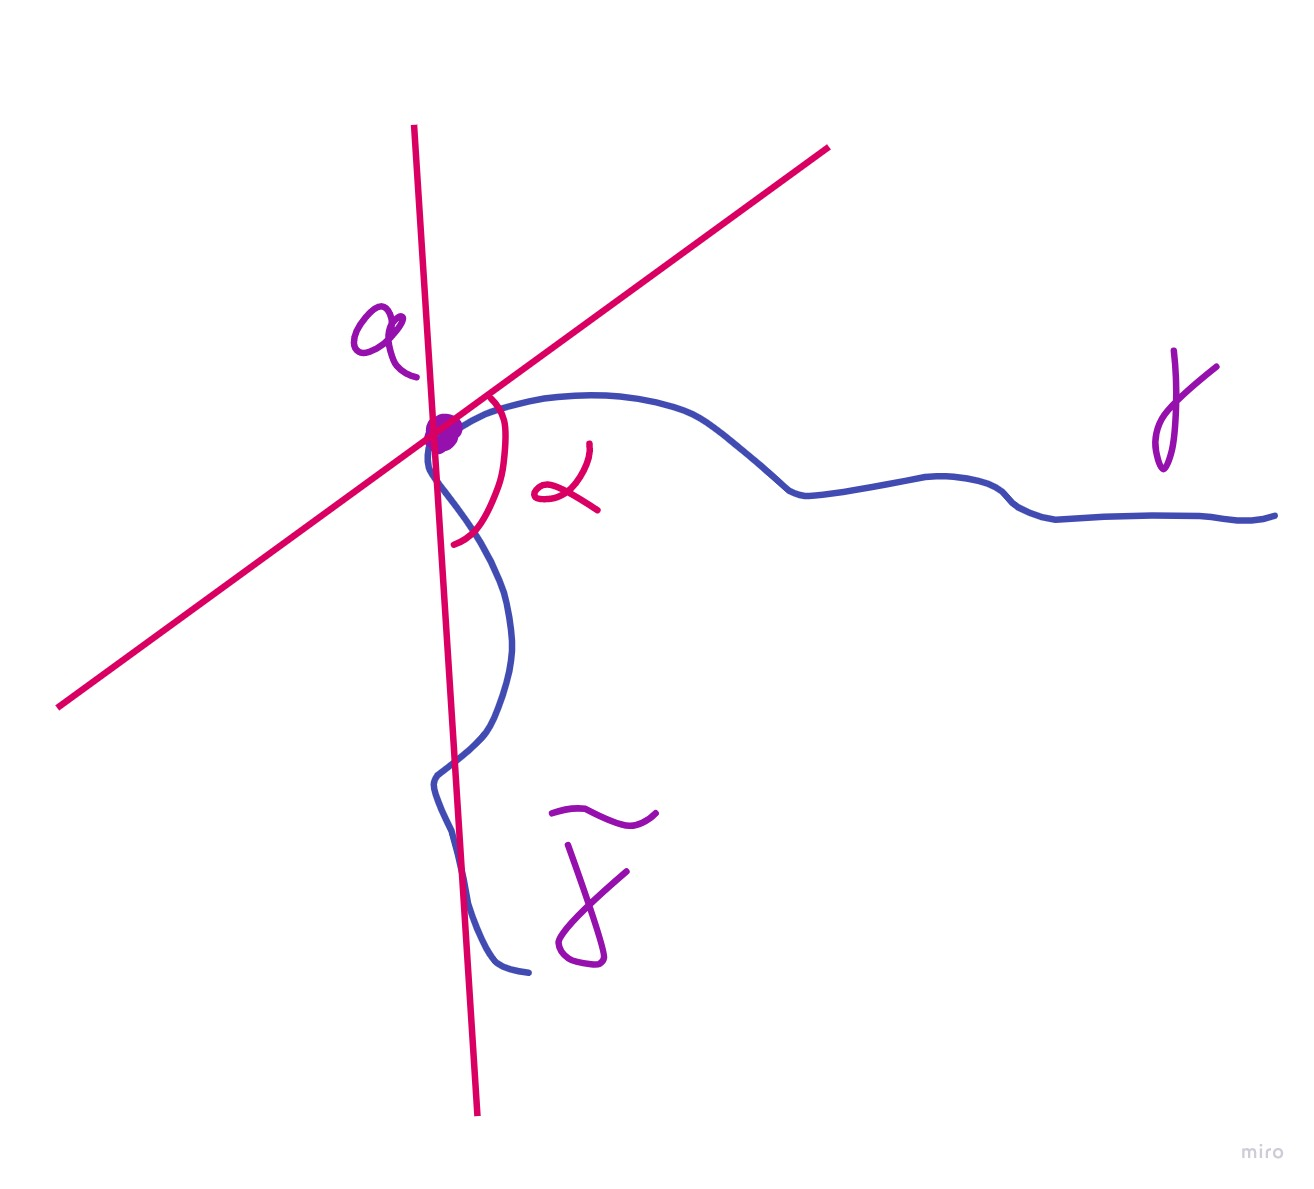
\includegraphics[width=8cm]{assets/04-functions-of-complex-variables/angle-between-curves.jpg}
    \end{center}

    $\arg \gamma'(0) - \arg \tilde{\gamma}'(0)$ - угол между кривым в $\Omega$.

    $\arg (f \circ \gamma)'(0) - \arg (f \circ \tilde{\gamma})'(0) = \arg f'(a)\gamma'(0) - \arg f'(a) \tilde{\gamma}'(0) =
    \arg \tilde{\gamma}'(0) - \arg \tilde{\gamma}'(0)$
\end{proof}

\begin{definition}
    $f : \Omega \to \mathbb{C}$ - однолистная, если $f \in H(\Omega)$ и
    инъекция.
\end{definition}

\begin{theorem}
    Если $f \in H(\Omega)$ и $f \neq const$, то $f(\Omega)$ - область.
\end{theorem}

\begin{proof}
    \begin{enumerate}
        \item {
            Линейная связность остаётся (т.к. при непрерывном отображении путь, соединяющий некоторые точки, под действием непрерывного отображения будет переходить в путь, соединяющий образы этих точек).
        }
        \item {
            Нужно проверить, что $f(\Omega)$ - открытое множество. Возьмём точку
            в образе и докажем, что она там лежит с некоторым шариком.

            $b \in f(\Omega) \Rightarrow \exists \, a \in \Omega \, : \, f(a) = b$.


            \begin{center}
                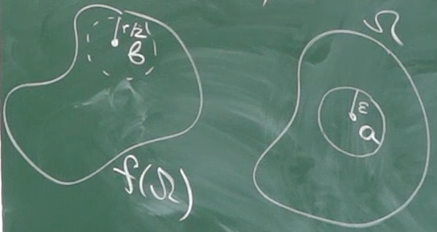
\includegraphics[width=10cm]{assets/04-functions-of-complex-variables/single-leaf-theorem.png}
            \end{center}

            Найдётся окружность $|z - a| < \varepsilon$, что $|f(z) - b| \neq 0$. Иначе бы на окружности радиуса $\frac{1}{n}$ нашлась точка $z_n$,
            такая, что $f(z_n) = b$, то $f \equiv b$ по теореме единственности, но $f \neq const$ по условию.

            $r = \min_{|z - a| = \varepsilon} |f(z) - b| > 0$. Мы хотим показать, что некоторый шарик $B_{\frac{r}{2}}(b) \subset f(\Omega)$, для этого посмотрим на уравнение $f(z) - w = 0$. Хотим понять, что такое уравнение
            имеет решение при $w$ близких к $b$ (а именно: $|w - b| < \frac{r}{2}$). Это и будет значить, что близкие к $b$ точки попадают в образ.

            Подставим всё в теорему Руше: $f(z) - w = (f(z) - b) + (b - w)$. Нужно, чтобы $|f(z) - b| > |b - w|$:

            $|f(z) - b| \geq r$ - т.к. $r$ -- это минимум данного выражения.

            $|b - w| \leq \frac{r}{2}$ -- т.к. мы берем $w$ из шарика $B_{\frac{r}{2}}(b)$.

            Итого получаем: $|f(z) - b| \geq r > \frac{r}{2} \geq |b - w| \rightarrow |f(z) - b| > |b-w|$ -- условия теоремы Руше выполнены, тогда $\mathcal{N}_{f(z) - w} = \mathcal{N}_{f(z) - b} \geq 1 \implies$ существует корень.

            Возьмём $|b-w| < \frac{r}{2}$ и всё выполнится.

            Получили, что $\{ |w-b| < \frac{r}{2} \} \subset f(\Omega) \Rightarrow f(\Omega)$ открытое.
        }
    \end{enumerate}
\end{proof}

\begin{consequence}
    Если $f$ однолистна, то $f$ конформное отображние $\Omega$ на $f(\Omega)$.
\end{consequence}

\begin{theorem}
    $f : \Omega \to \mathbb{C}$ однолистна. Тогда $f'(z) \neq 0 \, \forall \, z \in \Omega$.
\end{theorem}

\begin{proof}
    Пусть $f'(a) = 0$, $b = f(a)$. Возьмём $\varepsilon$ так, что
    $f(z) - b \neq 0$ при $|z - a| = \varepsilon$ и $r = \min_{|z - a| = \varepsilon} |f(z) - b| > 0$.

    \begin{center}
        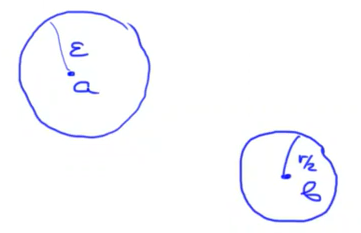
\includegraphics[width=6cm]{assets/04-functions-of-complex-variables/single-leaf-theorem-derivative-none-zero.png}
    \end{center}

    Смотрим на уравнение $f(z) - w = f(z) - b + b - w$. Мы выяснили, что
    $\mathcal{N}_{f - w} = \mathcal{N}_{f - b} \geqslant 2$, потому что
    $a$ - корень кратности $\geqslant 2$. Тогда $f(z) = w$ имеет хотя бы 2 решения. Но у нас инъекция, поэтому
    все решения с кратностью 2. Хотим показать, что тогда найдётся последовательность нулей производных,
    стремящаяся к точке $a$ и получить противоречие.

    Берём радиус $\frac{r}{2}$. $\{ |w - b| \leqslant \frac{r}{2} \} \subset f(\Omega)$.
    Берём $w_1, w_2, \ldots$ из этого круга. Значит $\exists \, z_1, \ldots$ из $|z - a| < \varepsilon$,
    $f(z_k) = w_k$ и $f'(z_k) = 0 \Rightarrow$ в $|z - a| \leqslant \varepsilon$ бесконечно много нулей
    $f'$. Значит у них есть предельная точка и тогда $f' \equiv 0 \Rightarrow f \equiv const$.
\end{proof}

\begin{remark}
    Обратное неверно. $f(z) = e^z, f'(z) = e^z \neq 0$, но нет однолистности.
\end{remark}

\begin{consequence}
    \begin{enumerate}
        \item {
            Конформное отображение сохраняет углы между кривыми

            \textit{Доказательство: } оно инъективно, а значит производная в ноль не обращается.
        }
        \item {
            Если $f(z) = c_0 + \frac{c_1}{z} + \frac{c_2}{z^2} + \ldots$ однолистна
            в окрестности $\infty$, то $c_1 \neq 0$.

            \textit{Доказательство: } $g(z) = f(\frac{1}{z})$ однолистна в проколотой окрестности нуля, в нуле можем доопределить, чтобы была голоморфность.

            \begin{center}
                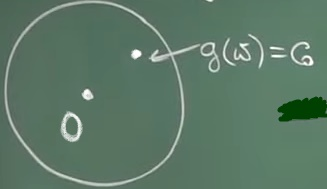
\includegraphics[width=7cm]{assets/04-functions-of-complex-variables/conf-func-consequence-2.jpg}
            \end{center}
            $g$ однолистна в меньшей не проколотой окрестности $\Rightarrow c_1 = g'(0) \neq 0$
        }
        \item {
            $f$ имеет полюс в точке $a$ и однолистна в проколотой окрестности точки $a$,
            тогда это полюс первого порядка.

            \textit{Доказательство: } пусть $g(z) = \frac{1}{f(z)}$ - однолистна в проколотой окрестности точки $a$.
            Можем доопределить нулём в точке $a$ и тогда будет голоморфность, $g(a) = 0$.

            Тогда $g$ однолистна в окрестности точки $a$, а значит $g'(a) \neq 0$, тогда $a$ -
            ноль первого порядка у $g$, а значит и ноль первого порядка у $f$.
        }
    \end{enumerate}
\end{consequence}

\begin{definition}
    $\Omega$ и $\tilde{\Omega}$ конформно эквивалентны, если $\exists \, f : \Omega \to \tilde{\Omega}$ - конформное отображение.

    \begin{remark}
        Это отношение эквивалентности.
    \end{remark}
\end{definition}

\begin{theorem}
    $\mathbb{C}$ и $\mathbb{D}$ не конформно эквивалентны.
\end{theorem}

\begin{proof}
    От противного. Пусть $f : \mathbb{C} \to \mathbb{D}$ - конформное отображение.

    Тогда $f \in H(\mathbb{C})$, $|f| \leqslant 1$. Тогда $f$ константа
    по теореме Луивилля. А это не биекция
\end{proof}

\begin{lemma}
    \textbf{Шварца}

    $f : \mathbb{D} \to \mathbb{D}$ голомофрная, $f(0) = 0$. Тогда:
    \begin{enumerate}
        \item $|f(z)| \leqslant |z| \forall \, z \in \mathbb{D}$
        \item Если для какого-то $a$, $|f(a)| = |a|$, то $f(z) = e^{i\phi} z$, где $\phi \in \mathbb{R}$
    \end{enumerate}
\end{lemma}

\begin{proof}
    \begin{enumerate}
        \item {
            Пусть $g(z) = \frac{f(z)}{z}$, в нуле устранимая особая точка, устраним - получим голоморфную в круге функцию.
            %TODO
            Согласно принципу максимума, в круге $|g(z)| \leqslant \max_{|z| = r} |g(z)| \leqslant \frac{1}{r} \rightarrow_{r \to 1-} 1$.
            И тогда $\frac{|f(z)|}{|z|} \leqslant 1$
        }
        \item {
            Знаем, что $|g(z)| \leqslant 1$ в $\mathbb{D}$. Если $|g(a)| = 1$, для $a \in \mathbb{D}$, то
            $a$ локальный максимум модуля и тогла, по принципу максимума, $g \equiv const \Rightarrow g(z) = e^{i\phi}$
        }
    \end{enumerate}

\end{proof}

\begin{theorem}
    \textbf{Римана о конфорных отображениях}

    $\Omega$ и $\tilde{\Omega}$ - односвязные области в $\bar{\mathbb{C}}$, причём их
    граница состоит больше, чем из одной точки (есть хотя бы какая-то кривая).
    Есть точка $z_0 \in \Omega, \tilde{z_0} \in \tilde{\Omega}$ и $\alpha \in \mathbb{R}$.

    Тогда существует единственное конформное отображение $f : \Omega \to \tilde{\Omega}$, такое,что
    $f(z_0) = \tilde{z_0}$ и $\arg f'(z_0) = \alpha$.
\end{theorem}

\begin{proof}
    \textit{Единственность}

    \begin{enumerate}
        \item {
            $\Omega = \tilde{\Omega} = \mathbb{D}, z_0 = \tilde{z_0} = 0$.

            Пусть $f : \mathbb{D} \to \mathbb{D}$, $f(0) = 0$ и $\arg f'(0) = \alpha$.
            По лемме Шварца для $f$ получаем, что $|f(z)| \leqslant |z| \, \forall z \in \mathbb{D}$.

            С другой стороны, $f^{-1} : \mathbb{D} \to \mathbb{D}$ тоже конфорное, $f^{-1}(0) = 0$, значит для
            неё тоже можно применить лемму Шварца. $|f^{-1}(z)| \leqslant |z| \Rightarrow |z| \leqslant |f(z)|$.

            Значит $|f(z)| = |z| \, \forall z \in \mathbb{D}$, тогда по лемме Шварца это поворот, то есть $f(z) = e^{i\phi}z$.

            Также мы знаем, что $f'(z) = e^{i\phi}$ и $\arg f'(0) = 0 \implies e^{i\phi} = 1$.
        }
        \item {
            $\Omega$ и $\tilde{\Omega}$ проивзольные. Пусть $f_1, f_2 \, : \, \Omega \to \tilde{\Omega}$ - конфорное.
            $f_i(z_0) = \tilde{z_0}$ и $\arg f_i' (z_0) = \alpha$, где $i \in \{1, 2\}$.

            Воспользуемся \textit{существованием}:

            \begin{enumerate}
                \item {
                    $\exists \phi : \mathbb{D} \rightarrow \Omega$ -- конформное, $\phi(0) = z_0$ и $\phi'(0) > 0$ (то есть, что $\arg \phi'(0) = 0$).
                }
                \item {
                    $\exists \psi : \tilde{\Omega} \rightarrow \mathbb{D}$ -- конформное, $\psi(\tilde{z_0}) = 0$ и $\arg \psi'(\tilde{z_0}) = -\alpha$.
                }
            \end{enumerate}

            Посмотрим на $g_i = \psi \circ f_i \circ \phi: \mathbb{D} \rightarrow \mathbb{D}$:

            \begin{enumerate}
                \item $g_i(0) = 0$
                \item {
                    $g_i'(0) = \psi'(f_i(\phi(0))) \cdot f_i'(\phi(0)) \cdot \phi'(0) = \psi'(\tilde{z_0}) \cdot f_i'(z_0) \cdot\phi'(0)$

                    $\arg g_i'(0) = -\alpha + \alpha + 0 = 0$ -- сумма аргументов множителей.
                }
            \end{enumerate}

            То есть мы получили, что $g_1$ и $g_2$ -- два комфорных отображения из круга в круг, переводящие ноль в ноль, и производную в нуле имеют с нулевым аргументом $\implies_{\text{по пункту (1)}} g_1 = g_2 = z$.

            Тогда восстановим $f_i$ и поймем, что они равны:

            $f_i(\phi(z)) = \psi^{-1}(g_i(z)) \implies f_i(z) = \psi^{-1}(g_i(\phi^{-1}(z))) \implies$ т.к. $g_1 = g_2$, то по полученной формуле $f_1 = f_2$.
        }
    \end{enumerate}
\end{proof}

\begin{consequence}
    \textbf{Обобщенная теорема Лиувилля}

    $f \in H(\mathbb{C})$ и $f$ не принимает значения на некоторой кривой $\gamma$. Тогда
    $f \equiv const$
\end{consequence}

\begin{proof}
    $\bar{\mathbb{C}} \setminus \gamma$ - односвязная область, с границей, состоящей из более чем одной точки.

    Тогда по теореме Римана о комформных отображениях существует $g : \bar{\mathbb{C}} \setminus \gamma \to \mathbb{D} \Rightarrow g \circ f \in H(\mathbb{C})$ и $g \circ f \subset \mathbb{D}$, то есть
    это ограниченная функция.

    Тогда по теореме Лиувилля (стандартной), $g \circ f$ - константа, значит
    $f(z) = g^{-1} (const) = const$.
\end{proof}

\begin{remark}
    \textbf{Малая теорема Пикара}

    Если $f \in H(\mathbb{C})$ не принимает 2 каких-то значения, то
    $f \equiv const$.
\end{remark}

\begin{example}
    $f(z) = e^z \neq 0$ - одно значение целая функция может не принимать.
\end{example}

\begin{consequence}
    Если $f$ мероморфна в $\mathbb{C}$ и не принимает 3 значения, то $f \equiv const$
\end{consequence}

\begin{proof}
    Пусть нет значений $a, b, c$. Сделаем из меромофрной - голоморфную, которая не принимает 2 значения.
    Пусть $c \neq \infty$, тогда $g(z) = \frac{1}{f(z) - c} \in H(\mathbb{C})$, но она не
    принимает значения $\frac{1}{a - c}$ и $\frac{1}{b - c}$, а тогда по малой теореме Пикара получаем, что $f \equiv const$.
\end{proof}

\begin{example}
    $f(z) = \tg z \neq \pm i$ - пример мероморфной функции, не принимающей 2 значения.
\end{example}

\begin{definition}
    $f(z) = \frac{az + b}{cz + d}$ - дробно-линейное отображение, $ad - bc \neq 0$.
\end{definition}

\begin{theorem}
    Если $f \in H(\bar{\mathbb{C}} \setminus \{z_0\})$ и однолистна, то $f$ дробно-линейное отображение.
\end{theorem}

\begin{proof}
    % $z_0$ - изолированная особая точка.

    \begin{enumerate}
        \item {
            $z_0$ -- существенная особая точка. Тогда по теореме Сохоцкого
            $Cl \, f \{ 0 < |z - z_0| < \varepsilon \} = \mathbb{C}$.

            Возьмём $b = f(a)$. Тогда $f(|z - a| < r)$ - открытое множество (т.к. $\{|z-a| < r\}$ -- открытое и $f$ -- однолистная).

            Более того, $f(|z - a| < r) \cap f(0 < |z - z_0| < \varepsilon) = \emptyset$ из однолистности.


            \begin{center}
                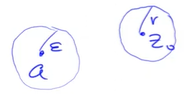
\includegraphics[width=5    cm]{assets/04-functions-of-complex-variables/fractional-linear-functions.png}
            \end{center}

            То же самое верно, если дописать замыкание: $f(|z - a| < r) \cap Cl \; f(0 < |z - z_0| < \varepsilon) = \emptyset$ --  противоречие (т.к. замыкание это все $\mathbb{C}$).
        }
        \item {
            $z_0 \neq \infty$ -- полюс. Тогда из однолистности это полюс первого порядка. А тогда
            $g(z) = f(z) - \frac{c}{z - z_0} \in H(\bar{\mathbb{C}}) \Rightarrow g(z) = const \Rightarrow f(z) = \frac{c}{z - z_0} + const$
        }
        \item {
            $z_0 = \infty$ -- полюс, тогда $g(z) = f(z) - cz \in H(\bar{\mathbb{C}}) \Rightarrow g(z) = const \Rightarrow f(z) = cz + const$.
        }
        \item {
            $z_0$ -- устранимая особая точка $\implies f \in H(\bar{\mathbb{C}}) \implies f \equiv const \implies$ нет однолистности $f$ -- противоречие.
        }
    \end{enumerate}
\end{proof}

\begin{consequence}
    Если функция $f \in H(\mathbb{C})$ и однолистная, то $f$ линейная.
\end{consequence}

\begin{proof}
    $z_0 = \infty$ в теореме.
\end{proof}

\Subsection{Производящие функции}

\begin{definition}
    Есть последовательность $a_0, a_1, \ldots$. Производящая функция последовательности
    $\mathcal{A}(z) = \sum_{n = 0}^{\infty} a_nz^n$.

    Мы хотим, чтобы ряд сходился при $|z| < R$ для какого-то $R > 0$
\end{definition}

\begin{example}
    \textbf{Задача о размене}

    Есть монетки $1, 2, 5, 10$ рублей. Интересуемся, каким количеством способов мы можем разменять $n$ рублей, если запас монет не ограничен, пусть это число равно $a_n$.

    Вместо формулы для этих коэффициентов будет искать формулу для ряда:

    $\mathcal{A}(z) := \sum_{n=0}^{\infty} a_n z^n$.

    Это будет равно:

    $\mathcal{A}(z) = (1 + z + z^2 + \ldots)(1 + z^2 + \ldots)(1 + z^5 + z^{10} + \ldots)(1 + z^{10} + z^{20} + \ldots)$ и
    раскроем все скобки.

    Коэффициент при $z^n = z^a \cdot z^{2b} \cdot z^{5c} \cdot z^{10d}$, где $a + 2b + 5c + 10d = n$.
    Тогда коэффициент $a_n$ -- число решений уравнения $a + 2b + 5c + 10d = n$ в неотрицательных целых числах.

    $\mathcal{A}(z) = \frac{1}{1 - z} \cdot \frac{1}{1 - z^2} \cdot \frac{1}{1 - z^5} \cdot \frac{1}{1 - z^{10}}$.
\end{example}

\begin{definition}
    $H \subset \mathbb{N}, \ p(n, H)$ - количество способов представить $n$ в виде суммы слагаемых из $H$.

    $\mathcal{F}_{H}(z) = \sum_{n=0}^{\infty} p(n, H) z^n = \prod_{k \in H} \frac{1}{1 - z^k}$

    Если каждое слагаемое можно брать $\leqslant m$, то $\prod_{k \in H} \underbrace{\frac{1 - z^{(m+1)k}}{1 - z^k}}_{=(1 + z^k + z^{2k} + \dots + z^{mk})}$
\end{definition}

\begin{definition}
    Число разбиений $n$ на натуральные слагаемые $p(n) = p(n, \mathbb{N})$.
\end{definition}

\begin{theorem}
    $f(z) = \sum_{n = 0}^{\infty} p(n) z^n = \prod_{k=1}^{\infty} \frac{1}{1 - z^k}$ -- сходится при $|z| < 1$
    и $p(n) = \frac{1}{2\pi i} \int_{|z| = r} \frac{f(z)}{z^{n + 1}} \, dz$ при $0 < r < 1$.
\end{theorem}

\begin{proof}
    $\ln \left (\prod_{k=1}^{\infty} \left | \frac{1}{1 - z^k} \right | \right ) = \sum_{k=1}^{\infty} -\ln |1 - z^k| = (*)$ -- покажем, что этот ряд сходится.

    \begin{enumerate}
        \item $\ln{(1 - t)} \geq -t - t^2 \implies -\ln{(1 - t)} \leq t + t^2$
        \item $\ln{|1 - z^k|} \geq \ln{(1 - |z|^k)} \implies -\ln{|1 - z^k|} \leq -\ln{(1 - |z|^k)} \leq |z|^k + |z|^{2k}$
    \end{enumerate}

    Из пункта (2) выше получаем, что $(*) \leq \sum_{k=1}^{\infty} |z|^k + \sum_{k=1}^{\infty} |z|^{2k} < +\infty$ -- справа от нер-ва сумма рядов сх-ся, тогда и $(*)$ тоже.

    Проверим, что аргумент ничего не испортит:

    % $\ln (1 + t) \geqslant t - t^2$ при $|t| < 1$. $\ln (1 - |z|^k) \geqslant |z|^k - |z|^{2k}$ и
    % $0 \leqslant -\ln |1 - z^k| \leqslant |z|^k + |z|^{2k}$.

    $\arg \left ( \frac{1}{1 - z^k} \right ) = -\arg (1 - z^k)$

    $|\arg (1 - z^k)| \leqslant \arcsin |z|^k \leqslant 2|z|^k$

    Действительно, аргумент ничего не портит.
\end{proof}

\begin{remark}
    \textbf{Теорема Харди-Рамануджана}

    $p(n) \sim \frac{1}{4n\sqrt{3}} e^{\pi \sqrt{\frac{2}{3}}\sqrt{n}}$
\end{remark}

\begin{theorem}
    \textbf{Эйлера}

    Количество разбиений $n$ на нечётные слагаемые равно количеству разбиений
    $n$ на различные слагаемые
\end{theorem}

\begin{proof}
    Для различных слагаемых $\prod_{k = 1}^{\infty} (1+z^k)$

    Для нечётных слагаемых $\prod_{k = 1}^{\infty} (\frac{1}{1 - z^{2k -1}})$.

    Хотим понять, что это одно и то же.$\prod_{k = 1}^{\infty} (\frac{1}{1 - z^{2k -1}}) =
    \frac{\prod_{n = 1}^{\infty} \frac{1}{1-z^n}}{\prod_{k = 1}^{\infty} \frac{1}{1-z^{2k}}} =
    \prod_{n = 1}^{\infty} \frac{1 - z^{2n}}{1 - z^n} = \prod_{n = 1}^{\infty} (1 + z^n)$
\end{proof}

\begin{example}
    $b_1b_2 \ldots b_k b_{k + 1} \ldots b_{2k}$ счастливый билет, если
    сумма первых $k$ равна сумме последних $k$.

    Пусть $a_n$ - количество $k$-значных чисел с суммой цифр $n$. То есть
    количество счастливых билетов $a_0^2 + a_1^2 + \ldots + a_{9k}^2$.

    Пусть $\mathcal{A}(z) = \sum_{n = 0}^{\infty} a_nz^n = (1 + z + z^2 + \ldots + z^9)^k$

    $\mathcal{A}(z) \cdot \mathcal{A}(\frac{1}{z})$ - здесь коэффициент перед $z^0$ - это $a_0^2 + a_1^2 + \ldots$.

    $\frac{1}{2\pi i} \int_{|z| = r} \frac{\mathcal{A}(z) \mathcal{A}\frac{1}{z}}{z} \, dz$ - количество счастливых билетов.
\end{example}

\begin{example}
    \textbf{Диагонализация степенных рядов}

    Пусть дана $f(w, z) = \sum_{n, k = 0}^{\infty} a_{nk} w^n z^k$, а мы хотим найти $g(w) = \sum_{n = 0}^{\infty} a_{nn} w^n$.

    Запишем $f(\frac{w}{z}, z) = \sum_{n, k = 0}^{\infty} a_{nk} \frac{w^n}{z^n} z^k$, видно, что нас интересует коэффициент перед $z_0$ (если мы его найдет, то получем ответ).


    То есть $g(w) = \frac{1}{2\pi i} \int_{|z| = r} \frac{f(\frac{w}{z}, z)}{z} \, dz = \frac{1}{2\pi i} \int_{|z| = r} \sum_{n, k = 0}^{\infty} a_{nk} w^n z^{k - n - 1} \, dz =$

    $= \frac{1}{2\pi i} \sum_{n, k = 0}^{\infty} w^n a_{nk} \underbrace{\int_{|z| = r} z^{k - n - 1} \, dz}_{=0, \text{ при } k \not = n, \ 2\pi i \text{ иначе}} = \frac{1}{2\pi i} \sum_{n = 0}^{\infty} w^n a_{nn} 2\pi i = g(w)$


    Чтобы можно было переставить интеграл и сумму, нужна равномерная сходимость. То есть нужно попасть строго внутрь круга сходимости ряда $\sum |a_{nk}| r^{k-1} \left |\frac{w}{z} \right |^n$.

    Пусть радиус сх-ти для $z$ и для $w$ равен $R$, тогда нужно, чтобы $r < R, \left|\frac{w}{r}\right| < R$.

    % Нужно $\left | \frac{w}{z} \right | < \rho$. Берём
    % радиус сходимости для $z$, для $w$, всё половиним, ещё на что-то умножаем.

    \bigskip

    Давайте теперь воспользуемся полученной схемой на конкретном примере:

    пусть $f(w, z) = \sum_{n, k = 0}^{\infty} \binom{n+k}{k}w^nz^k = \sum_{m = 0}^{\infty} \sum_{k = 0}^{m} \binom{m}{k} w^{m - k}z^k = \sum_{m = 0}^{\infty} (w + z)^m = \frac{1}{1 - w - z}$.


    Найдем $\frac{1}{2\pi i} \int_{|z| = r} \frac{f(\frac{w}{z}, z)}{z} \, dz = \frac{1}{2\pi i} \int_{|z| = r} \frac{dz}{z \left(1 - \frac{w}{z} - z\right)} = -\frac{1}{2\pi i} \int_{|z| = r} \frac{dz}{z^2 - z + w} = (*)$.

    Ищем нули знаменателя, получаем особые точки: $\frac{1 \pm \sqrt{1 - 4w}}{2}$.

    В контур попадает только $\frac{1 - \sqrt{1 - 4w}}{2}$, так как второй корень близок к $1$, а этот как раз к нулю.

    $(*) = - \res = -\frac{1}{2z - 1} \bigg |_{z = \frac{1 - \sqrt{1 - 4w}}{2}} = \frac{1}{\sqrt{1 - 4w}}$.

    Мы получили, что $\sum_{n=0}^{\infty} \binom{2n}{n} w^n = \frac{1}{\sqrt{1 - 4 w}}$.

\end{example}

\begin{definition}
    \textbf{Произведение Адамара}

    $\mathcal{A}(z) = \sum_{n = 0}^{\infty} a_nz^n$

    $\mathcal{B}(z) = \sum_{n=0}^{\infty} b_nz^n$

    $\mathcal{A} \circ \mathcal{B} (z) = \sum_{n = 0}^{\infty} a_nb_n z^n$
\end{definition}

\begin{example}
    Как находить произведение Адамара.

    $f(w, z) = \mathcal{A}(z) \mathcal{B}(w) = \sum_{n, k = 0}^{\infty} a_nb_kz^nw^k$.

    Нас интересует диагональ этой штуки.
\end{example}

\begin{theorem}
    Произведение Адамара рациональных функций -- рациональная функция
\end{theorem}

\begin{definition}
    Последовательность $\{a_n\}$ -- \textbf{квазимногочлен}, если

    $a_n = p_1(n)q_1^n + p_2(n)q_2^n + \ldots + p_k(n)q_k^n$,

    где $q_1, \ldots, q_k \in \mathbb{C}$, а $p_1, \ldots, p_k$ -- многочлены с комплексными коэффициентами.
\end{definition}

\begin{lemma}
    $\mathcal{A}(z) = \sum_{n=0}^{\infty} a_n z^n$ -- рациональная фукнция $\Leftrightarrow$ при больших $n \,: \, a_n$ -- квазимногочлен.
\end{lemma}

\begin{proof}
    \begin{enumerate}
        \item {
            $\Rightarrow$. Разложим рациональную функцию на простейшие, $\frac{1}{(1 - qz)^m}$ -- то есть на линейную комбинацию таких.

            $\frac{1}{(1 - z)^m} = \sum_{n = 0}^{\infty} \binom{n + m - 1}{m - 1} z^n$

            Тогда $\frac{1}{(1 - qz)^m} = \sum_{n = 0}^{\infty} \frac{(n + m - 1) \ldots (n + 1)}{(m - 1)!}q^nz^n$
        }
        \item {
            $\Leftarrow$. Достаточно понять, что $a_n = p(n) \cdot q^n$ имеет рациональную производящую функцию, а потом просто сложить в сумму.

            Индукция по степени многочлена:

            \begin{enumerate}
                \item {
                    База: $\deg = 0$, $a_n = q^n$ производящая функция $\frac{1}{1 - qz}$.
                }
                \item {
                    Переход: $d - 1 \rightarrow d$.

                    Возьмём конкретный многочлен степени $d$: $\tilde{p}(n) = \frac{(n + d)(n + d - 1) \ldots (n + 1)}{d!}$.

                    Для $b_n = \tilde{p}(n)q^n$ производящая функция $\frac{1}{(1 - qz)^{d + 1}}$.

                    Из $p(n)$ вычтем $c \cdot \tilde{p}(n)$ так, чтобы степень уменьшилась, тогда по предположению индукции -- все работает.
                }
            \end{enumerate}
        }
    \end{enumerate}
\end{proof}

\begin{example}
    \textbf{Метод Дарбу}

    $f(z) = \sum_{n = 0}^{\infty} a_n z^n$ сходится в круге $|z| < R$.

    Тогда при любом $r$, таком что $r < R$, ряд $\sum_{n = 0}^{\infty} a_n r^n$ -- сходится и $a_n r^n \rightarrow 0 \Rightarrow a_n = o(r^{-n})$.

    Пусть $R$ -- радиус сходимости $f(z) = \sum_{n = 0}^{\infty} a_n z^n$, тогда мы знаем, что на границе круга сходимости есть особая точка.

    Если особых точек конечное число и это полюсы (для простоты будем считать, что одна), то тогда возьмём эту точку и напишем главную часть ряда Лорана:

    $h(z) = \text{главная часть ряда Лорана для функции $f$ в точке $a$}$.

    Тогда $g(z) = f(z) - h(z)$ имеет устранимую особую точку $a$. Давайте устраним ее, тогда $g(z)$ голоморфна в точке $a$. Тогда скорее всего её радиус сходимости $\tilde{R} > R$.

    $g(z) = \sum_{n = 0}^{\infty} b_n z^n \Rightarrow b_n =  o((\tilde{R} - \varepsilon)^{-n})$

    $h(z) = \frac{c_1}{z - a} + \frac{c_2}{(z - a)^2} + \ldots + \frac{c_r}{(z - a)^r}$, где $r$ -- порядок полюса, у $h(z)$ можно явно выписать коэффициенты (самый быстрорастущий это последний).

    $\frac{1}{(z - a)^r} = \frac{1}{a^r \left(\frac{z}{a} - 1\right)^r} = \frac{(-1)^r}{a^r} \cdot \sum_{n = 0}^{\infty} \binom{n + r - 1}{r - 1} \left( \frac{z}{a} \right)^n$.

    Оценим биномиальный коэффициент: $\binom{n + r - 1}{r - 1} = \frac{(n + r - 1) \ldots (n + 1)}{(r - 1)!} \sim \frac{n^{r - 1}}{(r - 1)!}$.

    Тогда $a_n \sim c_r \cdot \frac{n^{r - 1}}{(r - 1)!} \cdot \frac{(-1)^r}{a^{n + r}}$.
\end{example}

\begin{theorem}
    Пусть $f \in H(|z| < R)$, где $R > 1$ и $f(1) \neq 0$.

    Пусть $\frac{f(z)}{(1 - z)^\alpha} = \sum_{n = 0}^{\infty} b_n z^n, \ \alpha \in \mathbb{R}, \ \alpha \neq 0, -1, -2 \ldots$

    Тогда $b_n \sim f(1) \cdot \binom{n + \alpha - 1}{n} \sim f(1) \cdot \frac{n^{\alpha - 1}}{\Gamma (\alpha)}$
\end{theorem}

\begin{proof}

    Возьмём $1 < r < R$ и разложим $f(z) = \sum_{n = 0}^{\infty} a_n z^n$.

    Ряд сходится в точке $z = r \Rightarrow a_n = o(r^{-n})$.

    $\frac{1}{(1 - z)^\alpha} = \sum_{n = 0}^{\infty} \underbrace{\binom{n + \alpha - 1}{n}}_{=\frac{(n + \alpha - 1)(n + \alpha - 2) \ldots \alpha}{n!}} z^n$.

    Получаем:

    $\frac{f(z)}{(1 - z)^\alpha} = \sum a_n z^n \cdot \sum \binom{n + \alpha - 1}{n} z^n$

    $b_n = a_n \binom{\alpha - 1}{0} + a_{n - 1}\binom{\alpha}{1} + \ldots + a_0 \binom{n + \alpha - 1}{n} = \binom{n + \alpha - 1}{n} (a_0 + \frac{n}{n + \alpha - 1} a_1 + \frac{n(n - 1)}{(n + \alpha - 1)(n + \alpha - 2)} a_2 + \ldots + (\ldots) \cdot a_n)$, где все коэффициенты при $a_i$ стремятся к $1$.

    Хотим сказать, что $b_n \sim \binom{n + \alpha - 1}{n} \cdot (a_0 + a_1 + \ldots + a_n) \sim \binom{n + \alpha - 1}{n} \cdot f(1) =$

    $= \frac{\alpha(\alpha - 1) \ldots (\alpha + n - 1)}{n!} f(1) \rightarrow \frac{n^{\alpha - 1}}{\Gamma(\alpha)} \cdot f(1)$ -- последний переход из формулы Эйлера-Гаусса.

    Осталось понять, что $\Delta_n = (a_0 + \frac{n}{n + \alpha - 1}a_1 + \frac{n(n - 1)}{(n + \alpha - 1)(n + \alpha -2)}a_2 + \ldots + (\ldots)\cdot a_n) - (a_0 + a_1 + \ldots +a_n) \rightarrow 0$.

    Мы знаем, что $a_n = \mathcal{O}(r^{-n}) \Rightarrow |a_n| \leqslant \frac{C}{r^n}$.

    Тогда $|\Delta_n| \leqslant
    \underbrace{|a_1| \left|\frac{n}{n + \alpha - 1} - 1\right| +
    |a_2| \left|\frac{n (n - 1)}{(n + \alpha - 1) (n + \alpha - 2)} - 1\right| +
    \ldots +
    |a_m| \left|(\ldots) - 1\right|}_{\text{конечное число слагаемых } \rightarrow 0} +$

    $+ \left(\frac{C}{r^{m + 1}} + \frac{C}{r^{m + 2}} + \ldots\right)$

    Подберём так $m$ чтобы $\sum \frac{C}{r^{m + i}} \leqslant \varepsilon$. И тогда всё выполнилось при больших $n$.
\end{proof}

\begin{example}
    \begin{enumerate}
        \item {
            $f(z) = \frac{\sqrt{2 - z}}{(1 - z)^2}$

            Здесь круг сходимости $|z| < 1$, особая точка $z = 1$ -- полюс второго порядка.

            Главная часть ряда Лорана: $\frac{a}{1 - z} + \frac{b}{(1 - z)^2} = -\frac{1}{2} \cdot \frac{1}{1 - z} + \frac{1}{(1 - z)^2}$.

            Здесь $b = \sqrt{2 - 1} = 1$, $a = \res_{z = 1} = ((1 - z)^2 f(z))' \bigg|_{z = 1} = (\sqrt{2 - z})' \bigg|_{z = 1} = \frac{-1}{2 \sqrt{2 - z}} \bigg|_{z = 1} = -\frac{1}{2}$.

            $g(z) = f(z) - \frac{1}{(1 - z)^2} + \frac{1}{2} \cdot \frac{1}{1 - z}$  -- голоморфна в $z = 1$, тогда $g \in H(|z| < 2)$.

            Пусть $f(z) = \sum_{n=0}^{\infty} a_n z^n, \ g(z) = \sum_{n=0}^{\infty} b_n z^n, \ b_n = o\left( \frac{1}{(2 - \varepsilon)^n} \right)$

            $a_n = b_n -\frac{1}{2} + n + 1 = n + \frac{1}{2} + o \left( \frac{1}{(2 - \varepsilon)^n} \right)$
        }
        \item {
            $f(z) = \frac{e^z}{\sqrt{1 - z}} = \sum_{n = 0}^{\infty} a_n z^n$, круг сходимости $|z| < 1$, но $z = 1$ не полюс, а точка ветвления.

            $g(z) = \frac{e^z}{\sqrt{1 - z}} - \frac{e}{\sqrt{1 - z}} = \frac{e}{\sqrt{1 - z}} (e^{z - 1} - 1) = \frac{e}{\sqrt{1 - z}} (1 - z) \underbrace{\frac{e^{z - 1} - 1}{1 - z}}_{=h(z) \text{, голоморфна в 1}} = e\sqrt{1 - z} h(z)$, где на самом деле $h(z) = \frac{1 + (z - 1) + \frac{(z - 1)^2}{2} + \ldots}{1 - z} \in H(\mathbb{C})$.

            $g(z) = \sum b_n z^n$, из теоремы имеем $b_n \sim h(1) \frac{n^{-\frac{3}{2}}}{\Gamma (\frac{1}{2})} = -\frac{1}{\sqrt{\pi} n \sqrt{n}}$

            $e \sqrt{1 - z} = e \sum_{n=0}^{\infty} c_n z^n$.

            Тогда $a_n = e \cdot c_n + b_n = \frac{e \cdot \binom{2n}{n}}{4^n} + b_n = e \cdot \underbrace{\frac{\binom{2n}{n}}{4^n}}_{\sim \frac{1}{\sqrt{\pi n}}} + \mathcal{O}\left(\frac{1}{\sqrt{n^3}}\right)$.

            $\sqrt{1 - 4z} = \sum_{n=0}^{\infty} \binom{2n}{n} z^n$ -- с одной из прошлый лекций. Тогда $\sqrt{1 - z} = \sum \binom{2n}{n} \frac{z^n}{4^n}$.

            И тогда $a_n = e \cdot \frac{\binom{2n}{n}}{4^n} + b_n = e \cdot \frac{\binom{2n}{n}}{4^n} + \mathcal{O}\left(\frac{1}{n^{\frac{3}{2}}}\right)$
        }
    \end{enumerate}
\end{example}

\begin{example}
    \textbf{Метод Лапласа}

    Есть $2k$-значный номер, интересуемся количеством таких номеров, что сумма первых $k$ знаков равна сумме последних $k$ (счастливые билеты).

    Пусть $a_k = $ количество $2k$ значных счастливых билетов.

    $a_k = \frac{1}{2\pi i} \int_{|z| = 1} \mathcal{A}(z) \mathcal{A}(\frac{1}{z}) \frac{dz}{z}$

    $\mathcal{A}(z) = (1 + z + z^2 + \ldots + z^9)^k = \left( \frac{1 - z^{10}}{1 - z} \right)^k$

    Тогда $a_k =
    \frac{1}{2 \pi i} \int_{|z| = 1} \left( \frac{(1 - z^{10})(1 - z^{-10})}{(1 - z)(1 - \frac{1}{z})} \right)^k \frac{dz}{z} =
    \frac{1}{2\pi i} \int_{|z| = 1} \left( \frac{2 - z^{10} - z^{-10}}{2 - z - \frac{1}{z}} \right)^k \frac{dz}{z} = (*)$

    Делаем замену: $z = e^{it}, \ dz = i \cdot e^{it} dt$.

    $(*) = \frac{1}{2\pi i} \int_{0}^{2\pi} \left( \frac{2 - e^{10 it} - e^{-10 it}}{2 - e^{it} - e^{-it}} \right)^k \frac{i e^{it}}{e^{it}} \, dt = $

    $= \frac{1}{2\pi} \int_{0}^{2\pi} \left( \frac{2 - 2 \cos{(10 t)}}{2 - 2\cos{t}} \right)^k \, dt = \frac{1}{2\pi} \int_{0}^{2\pi} \left( \frac{2\sin^2{(5 t)}}{2 \sin^2{\frac{t}{2}}} \right)^k \, dt =$

    Делаем доп. замену: $s = \frac{t}{2}, \ 1 - \cos{t} = 2 sin^2{\frac{t}{2}}$.

    $= \frac{1}{2\pi} \int_{0}^\pi 2\left( \frac{\sin {(10s)}}{\sin s} \right)^{2k} \, ds \underbrace{=}_{\text{т.е. симметрия отн. } \frac{\pi}{2}} \frac{2}{\pi} \int_{0}^{\frac{\pi}{2}} \left( \frac{\sin (10x)}{\sin x} \right)^{2k} ds$.


    Можно выловить скорость роста интеграла: поведение определено точкой максимума у $\frac{\sin{(10x)}}{\sin{x}}$.

    \begin{center}
        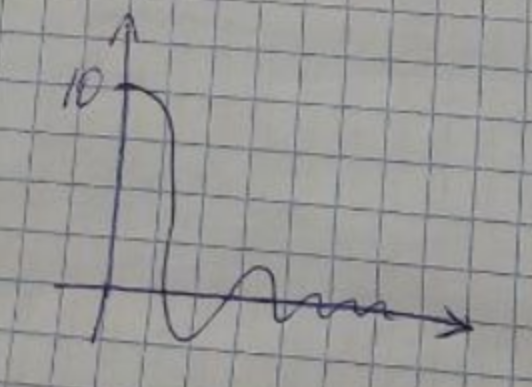
\includegraphics[width=6cm]{assets/04-functions-of-complex-variables/laplasian-method.png}
    \end{center}

    \begin{enumerate}
        \item В нуле максимум равен $10$
        \item В окрестности нуля разложим по Тейлору
        \item Остальное просто оценим
    \end{enumerate}

    $\int_{0}^{\frac{\pi}{2}} \left( \frac{\sin{(10x)}}{\sin{x}} \right)^k dx = \int_{0}^{\varepsilon} + \int_{\varepsilon}^{\frac{\pi}{2}}$


    \begin{enumerate}
        \item {
            Посмотрим на окрестность нуля.

            Раскладываем по Тейлору:

            $\frac{\sin{(10x)}}{\sin{x}} = \frac{10x - \frac{(10x)^3}{6} + \mathcal{O}(x^5)}{x - \frac{x^3}{3} + \mathcal{O}(x^3)} = 10 \cdot \frac{1 - \frac{100 x^2}{6} + \mathcal{O}(x^4)}{1 - \frac{x^2}{6} + \mathcal{O}(x^4)} =$

            $= 10 (1 - \frac{100}{6} x^2 + \mathcal{O}(x^4)) (1 + \frac{x^2}{6} + \mathcal{O}(x^4)) = 10 (1 - \frac{33}{2} x^2 + O(x^4))$

            Под интегралами у нас это степенная функция, поэтому распишем логарифм от нашего выражения:

            $\ln \frac{\sin(10x)}{\sin{x}} = \ln \left(10 (1 - \frac{33}{2} x^2 + O(x^4))\right)$

            $\left( \frac{\sin(10x)}{\sin{x}} \right)^{2k} = e^{2k \ln\left( 10 (1 - \frac{33}{2} x^2 + O(x^4)) \right)} = 10^{2k} \cdot e^{-33 k x^2} \cdot e^{\mathcal{O}(2k x^4)}$

            Подставим это в интеграл с $\varepsilon$:

            $k \varepsilon^4 \rightarrow 0$,

            $\int_{0}^{\varepsilon} 10^{2k} e^{-33k x^2} \underbrace{e^{\mathcal{O}(k x^4)}}_{= e^{\mathcal{O}(k \varepsilon^4)}, \text{ выберем $\varepsilon$ так, что } = 1 + \mathcal{O}(k \varepsilon^4)} = 10^{2k} \left( 1 + \mathcal{O}(k \varepsilon^4) \right) \int_{0}^{\varepsilon} e^{-33 k x^2} dx = (')$

            Делаем замену: $y = \sqrt{33k} x$.

            $(') = 10^{2k} \left(1 + \mathcal{O}(k \varepsilon^4)\right) \int_{0}^{\varepsilon \sqrt{33k}} e^{-y^2} \frac{1}{\sqrt{33k}} dy \sim 10^{2k} \frac{1}{\sqrt{33k}} \cdot \frac{\sqrt{\pi}}{2} = ('')$

            Хотим, чтобы $\varepsilon \sqrt{33} \rightarrow +\infty$, тогда $('') \rightarrow \int_{0}^{+\infty} = \frac{\sqrt{\pi}}{2}$.

            Для этого подойдет $\varepsilon = \sqrt{1}{k^{\frac{1}{3}}}$.
        }
        \item {
            Посмотрим на остальное.

            $\int_{\frac{\pi}{10}}^{\frac{\pi}{2}} \left( \frac{\sin{(10x)}}{\sin{x}} \right)^{2k} dx \leq \underbrace{\frac{\pi}{2}}_{\text{длина отрезка $\leq$ этого}} \left( \frac{1}{\sin{(\frac{\pi}{10})}} \right)^{2k}$

            если $\frac{\pi}{10}$ не подойдет, то немного подвинуть.

            Смотрим на вторую часть:

            $\int_{\varepsilon}^{\frac{\pi}{10}} \left( \frac{\sin{(10x)}}{\sin{x}} \right)^{2k} \underbrace{\leq}_{\text{т.к. функция убывает}} \frac{\pi}{10} \left(\frac{\sin{(10 \varepsilon)}}{\sin{\varepsilon}}\right)^{2k} \underbrace{=}_{\text{считали в предыдущем пункте}} \frac{\pi}{10} 10^{2k} \underbrace{e^{-33k \varepsilon^2}}_{\text{быстро убывает}} \underbrace{e^{\mathcal{O}(k \varepsilon^4)}}_{\sim 1}$
        }
    \end{enumerate}


    Метод работает в случае $\int_{a}^{b} \left(f(x)\right)^n$ и $n \rightarrow \infty$.
\end{example}